\documentclass[journal]{IEEEtran}

% =========================================================================
% Preamble & Package Inclusions
% =========================================================================
\usepackage{amsmath,amssymb,amsfonts,bm}
\usepackage{mathtools}
\usepackage{graphicx}
\usepackage{cite}
\usepackage{booktabs}
\usepackage{tabularx}
\usepackage{multirow}
\usepackage{multicol}
\usepackage{array}
\usepackage{algorithm}
\usepackage{algorithmic}
\usepackage{url}
\usepackage{microtype}
\usepackage{balance}

% Ensure correct column formatting for tabularx
\newcolumntype{Y}{>{\centering\arraybackslash}X}
\newcolumntype{L}{>{\raggedright\arraybackslash}X}

\begin{document}

% =========================================================================
% Paper Header & Title
% =========================================================================
\title{Resource-Efficient Multi-Objective Deep Q-Network for Decentralized Congestion Control in Dense V2X Networks}

\author{Gildong~Hong,~\IEEEmembership{Student~Member,~IEEE,}
        Cheolsoo~Kim,~\IEEEmembership{Member,~IEEE,}
        and~Younghee~Park,~\IEEEmembership{Senior~Member,~IEEE}%
\thanks{This work was supported in part by the National Research Foundation of Korea (NRF) Grant funded by the Korean Government (MSIT). \textit{(Corresponding author: Cheolsoo Kim.)}}%
\thanks{G. Hong and C. Kim are with the Department of Electrical and Computer Engineering, Seoul National University, Seoul 08826, South Korea (e-mail: gdhong@snu.ac.kr; cskim@snu.ac.kr).}%
\thanks{Y. Park is with the School of Electronic and Electrical Engineering, Korea University, Seoul 02841, South Korea (e-mail: yhpark@korea.ac.kr).}%
}

\markboth{IEEE Transactions on Wireless Communications,~Vol.~XX, No.~XX,~2026}%
{Hong \MakeLowercase{\textit{et al.}}: Resource-Efficient Multi-Objective Deep Q-Network for Decentralized Congestion Control}

\maketitle

% =========================================================================
% Abstract & Keywords
% =========================================================================
\begin{abstract}
In dense urban Vehicle-to-Everything (V2X) communication networks, broadcast storm problems and severe radio channel congestion critically degrade the timeliness of safety message delivery. Conventional standard Decentralized Congestion Control (DCC) protocols defined by the European Telecommunications Standards Institute (ETSI), such as ReactDCC and AdaptDCC, rely on static lookup tables or linear feedback mechanisms, which induce limit-cycle channel busy ratio (CBR) oscillations, packet bursts, and high collision probabilities in non-stationary traffic regimes. Moreover, monolithic single deep reinforcement learning (DRL) models suffer from severe capacity degradation across diverse traffic densities and often report inaccurate latency metrics by ignoring physical Medium Access Control (MAC) packet collisions. In this paper, we propose REMO-DQN, a resource-efficient multi-objective deep Q-network framework designed for real-time, closed-loop decentralized congestion control on vehicle on-board units (OBUs). REMO-DQN actively stabilizes channel utilization while ensuring optimal message freshness for time-critical vehicular safety applications.

REMO-DQN combines a two-block Residual Network (ResNet) feature extraction backbone, a detached Mixture-of-Experts (MoE) routing module comprising three domain-specialized experts (sparse, transitional, and severe congestion regimes), and a Dueling Q-head architecture with mean-centered value-advantage decomposition. To guarantee balanced optimization without expert collapse, we introduce a multi-objective reward function directly coupled with Carrier Sense Multiple Access with Collision Avoidance (CSMA/CA) collision attenuation and a squared coefficient of variation ($\text{CV}^2$) load-balancing regularization loss. Extensive empirical evaluations across 21 benchmark models (14 RL/DRL algorithms and 7 baseline/machine-learning schemes) under realistic Eclipse SUMO vehicular mobility and Nakagami-$m$ fading channels demonstrate that REMO-DQN achieves stable convergence within 80 episodes, completely suppresses CBR limit-cycle oscillations (mean CBR 0.3442, standard deviation 0.1008, 0.0\% violation of the 0.60 threshold), and defends a 73.41\% Packet Delivery Ratio (PDR) at an extreme density of 100~veh/km with merely a 3.13\%p drop. Furthermore, REMO-DQN achieves an average receiver-side Age of Information (AoI) of 373.21~ms, providing an 8.59-fold and 12.55-fold improvement over AdaptDCC and fixed 10~Hz transmission, respectively, while requiring only 3.8M MACs, 350K parameters, and 1.2~ms inference latency on an ARM Cortex MCU. These results confirm that REMO-DQN delivers an optimal balance between transmission reliability, computational efficiency, and channel stability.
\end{abstract}

\begin{IEEEkeywords}
Vehicle-to-Everything (V2X), Decentralized Congestion Control (DCC), Deep Reinforcement Learning (DRL), Mixture of Experts (MoE), Dueling DQN, Age of Information (AoI), Packet Delivery Ratio (PDR), Residual Connection (ResNet).
\end{IEEEkeywords}

\IEEEpeerreviewmaketitle

% =========================================================================
% Section I: Introduction
% =========================================================================
\section{Introduction}
\IEEEPARstart{W}{ith} the ongoing advancement of Connected and Autonomous Vehicles (CAVs), Vehicle-to-Everything (V2X) communication and Vehicular Ad-hoc Networks (VANETs) serve as fundamental infrastructure for Cooperative Intelligent Transport Systems (C-ITS) \cite{Arena2019Overview, Kenney2011DSRC}. In V2X environments, vehicles periodically broadcast Cooperative Awareness Messages (CAMs) or Basic Safety Messages (BSMs) containing kinematic variables such as positioning, velocity, heading, and acceleration to establish mutual situational awareness and prevent traffic collisions \cite{ETSI_EN_302_637_2, SAE_J2945_1}. However, in dense urban intersections and highway bottlenecks, hundreds of vehicles simultaneously contend for access over the shared 5.9~GHz Dedicated Short-Range Communications (DSRC) and C-V2X control channel (CCH) \cite{ETSI_TS_102_687}. This uncoordinated broadcasting leads to acute wireless channel saturation, severe packet collisions, and transmission delays, which degrade the safety guarantees of time-critical vehicular applications \cite{Zheng2022Age, Liu2024Age}. Consequently, establishing robust Decentralized Congestion Control (DCC) mechanisms that regulate channel load while preserving message freshness has become an urgent technical challenge.

Standard ETSI DCC protocols \cite{ETSI_TS_102_687, ETSI_TS_103_175}, namely reactive control (ReactDCC) and adaptive linear control (AdaptDCC), adjust packet generation intervals and transmit power according to local channel busy ratio (CBR) measurements. However, ReactDCC uses rigid finite state machines (FSM) with static lookup tables, causing sharp parameter transitions and limit-cycle CBR oscillations around congestion thresholds \cite{Bansal2013LIMERIC}. AdaptDCC mitigates step-wise fluctuations via linear proportional-integral feedback; nonetheless, it struggles to adapt to non-linear mobility dynamics and group-synchronized burst transmissions in dense vehicular regimes \cite{Ye2019Deep}. Crucially, both standard protocols focus solely on channel occupancy regulation while ignoring receiver-side Age of Information (AoI) and Medium Access Control (MAC) packet loss dynamics. When transmission frequency is increased naively without verifying reception success, channel congestion spikes, inducing consecutive packet collisions and precipitating a ``Fake AoI'' paradox where transmitter-side generation rates appear optimal while receiver-side information staleness severely collapses \cite{Zheng2022Age}.

To overcome the rigidity of rule-based protocols, machine learning and deep reinforcement learning (DRL) techniques have been applied to wireless resource allocation \cite{Hu2021Deep, Wang2023Multi, Mnih2015Human}. Value-based and policy-based algorithms, including Deep Q-Networks (DQN), Proximal Policy Optimization (PPO), Soft Actor-Critic (SAC), Deep Deterministic Policy Gradient (DDPG), and Multi-Agent PPO (MAPPO), have been explored for vehicular power and rate control \cite{VanHasselt2016Deep, Wang2016Dueling, Yu2022Surprising, Lowe2017Multi, Rashid2018QMIX}. However, previous studies exhibit major limitations. First, existing literature lacks extensive, standardized empirical benchmarks evaluating diverse RL families under identical physical (PHY) and MAC layer constraints. Second, vehicular environments exhibit non-stationary multi-modal traffic phases, ranging from sparse rural roads to ultra-dense urban intersections. Monolithic neural networks sharing a single parameter set suffer from parameter interference and catastrophic forgetting across disparate traffic regimes. Third, continuous actor-critic models and sequence transformers such as Decision Transformer \cite{Chen2021Decision, Janner2021Offline} incur high sample complexity, unstable gradient variance, and quadratic computational overhead, violating the stringent sub-millisecond real-time execution budget of embedded vehicle On-Board Units (OBUs).

To address these challenges, we introduce REMO-DQN, an integrated modular framework combining residual representation learning, conditional computation via Mixture of Experts (MoE), and Dueling Q-value decomposition. The proposed architecture uses a 2-block ResNet backbone to extract high-order latent features from 5-dimensional continuous state observations without vanishing gradients. A detached Softmax gating router dynamically directs execution across three specialized Dueling Q-expert sub-networks dedicated to sparse, transitional, and severe congestion regimes \cite{Shazeer2017Outrageously, Xu2025Mixture}. By decoupling the state value $V(\mathbf{s})$ from action advantages $A(\mathbf{s}, a)$ with mean-centering and applying a squared coefficient of variation ($\text{CV}^2$) load-balancing auxiliary loss, REMO-DQN achieves stable policy convergence while preventing expert collapse. Furthermore, the multi-objective reward formulation integrates physical MAC packet collision penalties, directly resolving the Fake AoI distortion.

The main contributions of this paper are summarized as follows:
\begin{itemize}
    \item \textbf{Multi-Model Empirical Benchmark:} We construct an end-to-end simulation framework integrating Eclipse SUMO micro-mobility and Nakagami-$m$ fading channels, conducting an empirical evaluation across 14 RL/DRL algorithms and 7 baseline schemes optimized via the Optuna framework.
    \item \textbf{CBR Flapping Suppression and PDR Defense:} REMO-DQN eliminates standard DCC limit-cycle oscillations, maintaining a stable mean CBR of 0.3442 with standard deviation 0.1008 and zero violation of the 0.60 threshold. At a vehicle density of 100~veh/km, REMO-DQN defends a 73.41\% PDR, representing a 3.13\%p decrease from 76.54\% at 10~veh/km, whereas conventional schemes degrade by 74--91\%p.
    \item \textbf{True AoI Freshness Optimization:} By coupling reward signals with physical CSMA/CA MAC collision dynamics, REMO-DQN achieves a network average AoI of 373.21~ms across all density domains, outperforming AdaptDCC with 3,205.96~ms and Fixed 10~Hz with 4,682.51~ms by 8.59-fold and 12.55-fold, respectively.
    \item \textbf{OBU Hardware Feasibility and Latency Profiling:} We evaluate the computational complexity on target ARM Cortex embedded hardware, confirming that REMO-DQN requires 3.8M MACs, 350K parameters, 1.4~MB memory, and 1.2~ms inference latency, occupying 1.2\% of the 100~ms DCC operational window.
\end{itemize}

The remainder of this paper is organized as follows. Section~II reviews related works on standard DCC, DRL-based resource allocation, and MoE architectures. Section~III details the system model, Dec-MDP problem formulation, REMO-DQN architecture, and training algorithm. Section~IV describes the dynamic cross-layer operational workflow. Section~V presents extensive simulation results across seven quantitative evaluation metrics. Finally, Section~VI concludes the paper and outlines future directions.

% =========================================================================
% Section II: Related Works
% =========================================================================
\section{Related Works}
In this section, we examine prior research on vehicular congestion control and wireless resource management. We analyze standard ETSI/SAE DCC protocols, single-agent and multi-agent reinforcement learning methods, and recent advances in MoE-enabled wireless networks, establishing the structural distinctions of REMO-DQN.

\subsection{Standard V2X Decentralized Congestion Control Protocols}
V2X communication standards established by ETSI and SAE specify periodic broadcasting of safety beacons (CAM and BSM) over the 5.9~GHz ITS band to ensure cooperative awareness \cite{Arena2019Overview, Kenney2011DSRC, ETSI_EN_302_637_2, SAE_J2945_1}. To mitigate channel saturation in dense topologies, the DCC sublayer operating above the IEEE 802.11p/bd and C-V2X MAC layers modulates transmission parameters across three primary dimensions: Transmit Power Control (TPC), Transmit Duty-cycle/Rate Control (TDC/TRC), and Transmit Datarate Control (DRC), aiming to bound channel occupancy below a target threshold ($\text{CBR}_{\text{target}} \approx 0.60$) \cite{ETSI_TS_102_687, ETSI_TS_103_175}. Additionally, Enhanced Distributed Channel Access (EDCA) prioritizes messages across four Access Categories (AC\_VO, AC\_VI, AC\_BE, AC\_BK). In dense vehicular scenarios, strict parameter modulation becomes necessary to prevent packet loss. Without coordinated access, broadcast traffic rapidly congests the shared radio medium, degrading communication reliability.

ReactDCC \cite{ETSI_TS_103_175} adopts an FSM that transitions among Relaxed, Active, and Restrictive states based on measured $\text{CBR}_t$:
\begin{equation}
\label{eq:react_dcc}
\text{State}_{t+1} = \begin{cases} 
\text{Relaxed}, & \text{if } \text{CBR}_t < \text{CBR}_{\text{min}}, \\ 
\text{Active}_k, & \text{if } \text{CBR}_k \le \text{CBR}_t < \text{CBR}_{k+1}, \\ 
\text{Restrictive}, & \text{if } \text{CBR}_t \ge \text{CBR}_{\text{max}}. 
\end{cases}
\end{equation}
Upon state entry, generation interval $T_{\text{GenCam}} \in [100, 1000]\text{ ms}$ and transmit power $P_{\text{tx}} \in [0, 33]\text{ dBm}$ are switched discretely. Despite hysteresis timers, this step-wise switching causes synchronized parameter transitions across neighboring vehicles, inducing limit-cycle CBR oscillations and packet transmission bursts \cite{Bansal2013LIMERIC}. When channel load crosses threshold boundaries, adjacent vehicles transition simultaneously into restrictive states, causing abrupt drops in message dissemination. As traffic disperses, vehicles rapidly revert to active states, triggering recurring congestion cycles.

To smooth these fluctuations, AdaptDCC (ETSI TS 102 687 Annex C) and LIMERIC employ linear feedback adjustment \cite{Bansal2013LIMERIC}:
\begin{align}
\label{eq:adapt_dcc_t}
T_{\text{GenCam}}(k) &= T_{\text{GenCam}}(k-1) + \beta \left( \text{CBR}_{\text{smooth}}(k) - \text{CBR}_{\text{target}} \right), \\
\label{eq:adapt_dcc_cbr}
\text{CBR}_{\text{smooth}}(k) &= (1 - w)\text{CBR}_{\text{smooth}}(k-1) + w\text{CBR}(k),
\end{align}
where $\beta$ is an adaptation gain and $w$ is an exponential smoothing factor. Although linear feedback reduces abrupt steps, fixed gains cannot accommodate non-linear spatial traffic dynamics, leading to sluggish adaptation during rapid vehicle influx and recurring channel overshoots \cite{Zheng2022Age, Ye2019Deep}. Crucially, both standard protocols regulate CBR blindly without incorporating physical packet collisions or true receiver-side AoI. When packets collide, standard DCC fails to distinguish channel noise from spatial contention, often worsening latency. Consequently, conventional standard DCC mechanisms cannot guarantee reliable safety message delivery under dense vehicular traffic regimes.

\subsection{Single-Agent DRL for Wireless Resource Management}
To overcome rule-based rigidity, deep reinforcement learning has been widely investigated for wireless resource allocation \cite{Ye2019Deep, Hu2021Deep, Mnih2015Human}. Formulated under Markov Decision Processes (MDPs), value-based DQN approximates optimal action-values by minimizing the temporal difference (TD) loss:
\begin{equation}
\label{eq:dqn_loss}
\mathcal{L}(\theta) = \mathbb{E}_{(\mathbf{s}, a, r, \mathbf{s}')} \left[ \left( r + \gamma \max_{a'} Q(\mathbf{s}', a'; \theta^-) - Q(\mathbf{s}, a; \theta) \right)^2 \right],
\end{equation}
where Double DQN \cite{VanHasselt2016Deep} and Dueling DQN \cite{Wang2016Dueling} address overestimation bias and state-action value separation. Ye \textit{et al.} \cite{Ye2019Deep} applied DQN for distributed V2V spectrum and power allocation, improving transmission capacity. Zheng \textit{et al.} \cite{Zheng2022Age} developed a state-history DQN for AoI-oriented congestion control. These value-based approaches demonstrate improved channel efficiency over heuristic rules. However, standard DQN formulations struggle under dynamic traffic conditions due to monolithic state representations.

Continuous action management has been pursued via policy gradient and actor-critic algorithms \cite{Hu2021Deep, Liu2024Age}. PPO minimizes a clipped surrogate objective to bound policy updates:
\begin{align}
\label{eq:ppo_clip}
\mathcal{L}^{\text{CLIP}}(\theta) &= \hat{\mathbb{E}}_t \left[ \min\left( \rho_t(\theta)\hat{A}_t, \, \text{clip}(\rho_t(\theta), 1-\epsilon, 1+\epsilon)\hat{A}_t \right) \right], \\
\label{eq:ppo_rho}
\rho_t(\theta) &= \frac{\pi_\theta(a_t|\mathbf{s}_t)}{\pi_{\theta_{\text{old}}}(a_t|\mathbf{s}_t)},
\end{align}
while SAC maximizes expected return alongside policy entropy $\mathcal{H}(\pi(\cdot|\mathbf{s}_t))$ \cite{Liu2024Age}:
\begin{equation}
\label{eq:sac_obj}
J(\pi) = \sum_{t=0}^T \mathbb{E}_{(\mathbf{s}_t, a_t)} \left[ r(\mathbf{s}_t, a_t) + \alpha \mathcal{H}(\pi(\cdot|\mathbf{s}_t)) \right].
\end{equation}
Hu \textit{et al.} \cite{Hu2021Deep} used DDPG for cross-layer V2X resource scheduling, while Liu \textit{et al.} \cite{Liu2024Age} investigated PPO and SAC for AoI-energy optimization. In vehicular settings, continuous policy exploration introduces high training variance. Furthermore, actor-critic models often experience policy instability when deployed on resource-constrained embedded microcontrollers.

Nonetheless, single-agent monolithic DRL exhibits distinct drawbacks when applied to vehicular decentralized congestion control. First, extreme channel non-stationarity caused by rapid topology alterations severely destabilizes policy gradients during distributed deployment. Second, sharing a single monolithic network parameter set across sparse and saturated traffic regimes triggers catastrophic forgetting and representational interference. Third, continuous actor-critic exploration suffers from pronounced sample inefficiency, requiring excessive interaction episodes to reach policy convergence. Fourth, single-objective reward formulations fail to capture the multi-dimensional Pareto boundary between CBR regulation, message freshness, and collision-induced packet loss. Consequently, specialized modular architectures are essential to overcome the representational bottlenecks of monolithic learning models.

% =========================================================================
% Table I: Literature Comparison (table*)
% =========================================================================
\begin{table*}[t]
\caption{Comparison of Related Studies on V2X Congestion Control and RL Frameworks}
\label{tab:lit_comparison}
\centering
\scriptsize
\begin{tabularx}{\textwidth}{>{\centering\arraybackslash}p{2.2cm} L L >{\centering\arraybackslash}p{2.0cm} >{\centering\arraybackslash}p{2.8cm}}
\toprule
\textbf{Reference} & \textbf{Optimization Target} & \textbf{RL Algorithm Used} & \textbf{Baselines} & \textbf{MoE / Ensemble} \\
\midrule
\cite{ETSI_TS_102_687, ETSI_TS_103_175} & CBR Stability & N/A (Static Rule-based FSM / PI) & 2 & No \\
\cite{Ye2019Deep} & V2V Capacity \& Latency & Vanilla DQN & 3 & No \\
\cite{Hu2021Deep} & PDR \& Throughput & DDPG & 4 & No \\
\cite{Zheng2022Age} & AoI \& CBR Trade-off & Deep Q-Learning & 3 & No \\
\cite{Wang2023Multi} & PDR \& Power Efficiency & MAPPO (CTDE) & 4 & No \\
\cite{Bhattacharyya2024Hybrid} & AoI \& Channel Load & Tabular Q-Learning & 3 & No \\
\cite{Liu2024Age} & AoI \& Energy Consumption & SAC / PPO & 5 & No \\
\cite{Kang2024Task} & Edge Latency \& Resource Cost & Meta-RL + Task-Oriented MoE & 4 & Yes \\
\cite{Xu2025Mixture} & Generalization \& Edge Efficiency & Survey on MoE + Wireless DRL & N/A & Yes \\
\cite{Du2025Generative} & Slicing Resource Allocation & Generative AI + MoE & 3 & Yes \\
\cite{Park2025Ensemble} & PDR \& Channel Load & Ensemble Deep Q-Learning & 3 & Yes \\
\cite{Zhang2026Generalizable} & MAC Throughput \& Protocol Adapt. & Meta-RL + MoE Router & 4 & Yes \\
\midrule
\textbf{Proposed REMO-DQN} & \textbf{CBR Stability, AoI Freshness, PDR, Energy, Latency} & \textbf{ResNet-MoE-Dueling DQN} & \textbf{21 (14 RL + 7 Base)} & \textbf{Yes (3 Dueling Experts)} \\
\bottomrule
\end{tabularx}
\end{table*}

\subsection{Multi-Agent DRL and Sequence Models in V2X}
Cooperative multi-agent reinforcement learning (MADRL) under Centralized Training with Decentralized Execution (CTDE) has been studied to coordinate multi-vehicle interactions \cite{Wang2023Multi, Yu2022Surprising, Lowe2017Multi}. MAPPO \cite{Yu2022Surprising} and MADDPG \cite{Lowe2017Multi} use centralized critics evaluating global state vectors $S = (\mathbf{s}_1, \dots, \mathbf{s}_N)$ during training while executing decentralized actor policies on local observations. Value factorization methods like QMIX \cite{Rashid2018QMIX} enforce monotonic joint value constraints. Furthermore, casting RL as conditional sequence modeling via Decision Transformer (DT) \cite{Chen2021Decision} and Trajectory Transformer \cite{Janner2021Offline} has emerged:
\begin{equation}
\label{eq:dt_seq}
\tau = \left( \hat{R}_1, \mathbf{s}_1, a_1, \hat{R}_2, \mathbf{s}_2, a_2, \dots, \hat{R}_T, \mathbf{s}_T, a_T \right),
\end{equation}
where autoregressive attention generates actions conditioned on return-to-go $\hat{R}_t$.

However, deploying MADRL and transformer sequence models onto embedded vehicular OBUs encounters severe practical bottlenecks. First, inter-vehicle signaling exchanges add heavy wireless overhead onto the already saturated 5.9~GHz control channel, exacerbating packet collision risks. Second, dynamic node entrance and exit in urban intersections violate fixed-agent cardinality assumptions required by centralized critics. Third, the quadratic computational complexity $\mathcal{O}(T^2)$ of autoregressive attention introduces excessive inference latency on resource-constrained microcontrollers. Fourth, global state estimation degrades rapidly when localized packet loss corrupts multi-hop state dissemination. Therefore, ultra-lightweight decentralized execution operating solely on local sensory observations is mandatory for real-time vehicular control.

\subsection{Latest MoE-Enabled Wireless Networks (2024--2026)}
Mixture of Experts (MoE) architectures provide conditional computation by activating specialized sub-networks per input instance without expanding total inference floating-point operations \cite{Shazeer2017Outrageously}:
\begin{equation}
\label{eq:moe_convex}
\mathbf{y} = \sum_{k=1}^K g_k(\mathbf{x}) E_k(\mathbf{x}), \quad \text{s.t.} \quad \sum_{k=1}^K g_k(\mathbf{x}) = 1, \quad g_k(\mathbf{x}) \ge 0.
\end{equation}
Recent studies from 2024 to 2026 have explored MoE for wireless edge networks \cite{Xu2025Mixture, Zhang2026Generalizable, Kang2024Task, Du2025Generative, Park2025Ensemble, Bhattacharyya2024Hybrid}. Xu \textit{et al.} \cite{Xu2025Mixture} surveyed MoE paradigms for decentralized generative AI and wireless RL. Zhang \textit{et al.} \cite{Zhang2026Generalizable} developed meta-RL MoE routers for generalizable multiple access. Kang \textit{et al.} \cite{Kang2024Task} formulated task-oriented MoE for multi-modal edge slicing, and Du \textit{et al.} \cite{Du2025Generative} applied MoE to generative network slicing. Park and Kim \cite{Park2025Ensemble} explored ensemble Q-learning for channel regulation.

Despite these contributions, existing MoE wireless architectures predominantly target base stations or edge cloud servers, resulting in multi-million parameter footprints that cannot run on vehicular microcontrollers. Moreover, prior formulations assume idealized radio channels and omit physical CSMA/CA MAC collision dynamics. In contrast, REMO-DQN delivers an embedded MCU-friendly design with 350K parameters and 1.2~ms forward inference latency. Furthermore, the framework incorporates an explicit multi-objective reward formulation directly coupled with physical collision loss and coordinates three domain-specific experts validated against 21 benchmark models. Table~\ref{tab:lit_comparison} summarizes the structural differences across related literature.

% =========================================================================
% Section III: System Model and Proposed REMO-DQN Architecture
% =========================================================================
\section{System Model and REMO-DQN Architecture}
In this section, we formulate the network topology, physical radio propagation, CSMA/CA MAC contention mechanics, ETSI dynamic packet generation rules, and the Dec-MDP framework. We then present the complete REMO-DQN neural architecture and its optimization algorithm.

\subsection{Network and Communication System Model}
\subsubsection{Network Topology and Time-Slotting}
We consider a vehicular ad-hoc network over an urban arterial road network operating in discrete time slots with fundamental control step $\Delta T_{\text{step}} = 100\text{ ms}$ ($0.1\text{ s}$). At time slot $t \in \{0, 1, \dots, T_{\text{end}}\}$, let $\mathcal{V}(t) = \{v_1, \dots, v_{N(t)}\}$ denote the set of active vehicles, where $N(t) = |\mathcal{V}(t)|$. Each vehicle $i \in \mathcal{V}(t)$ is equipped with a GNSS receiver and an IEEE 802.11p OBU, maintaining kinematics $\mathbf{p}_i(t) = (x_i(t), y_i(t)) \in \mathbb{R}^2$, speed $v_i(t)$, and heading angle $\theta_i(t)$. The Euclidean spatial distance between vehicles $i$ and $j$ is given by:
\begin{equation}
\label{eq:distance}
d_{ij}(t) = \|\mathbf{p}_i(t) - \mathbf{p}_j(t)\|_2 = \sqrt{(x_i(t) - x_j(t))^2 + (y_i(t) - y_j(t))^2}.
\end{equation}
Equipped with omni-directional antennas, vehicles have a safety communication range $R_{\text{comm}} = 300\text{ m}$ and an energy sensing range $R_{\text{sense}} = 500\text{ m}$. The active communication and sensing neighbor sets are defined as:
\begin{align}
\label{eq:neighbors}
\mathcal{N}_{\text{comm}}(i, t) &= \{j \in \mathcal{V}(t) \mid j \neq i, d_{ij}(t) \le R_{\text{comm}}\}, \\
\mathcal{N}_{\text{sense}}(i, t) &= \{j \in \mathcal{V}(t) \mid j \neq i, d_{ij}(t) \le R_{\text{sense}}\}.
\end{align}

\subsubsection{Physical Layer Radio Propagation Model}
Vehicular transmissions operate over the 5.9~GHz CCH ($f_c = 5.9\text{ GHz}$) with bandwidth $B = 10\text{ MHz}$. BPSK $1/2$ modulation provides a nominal data rate $R_{\text{data}} = 3\text{ Mbps}$. Standard CAM beacons have fixed payload $L_{\text{CAM}} = 280\text{ Bytes} = 2240\text{ bits}$. The packet air-time transmission duration $T_{\text{tx}}$ is:
\begin{equation}
\label{eq:airtime}
T_{\text{tx}} = \frac{L_{\text{CAM}} \times 8}{R_{\text{data}}} = \frac{2240\text{ bits}}{3 \times 10^6\text{ bps}} \approx 0.74667\text{ ms}.
\end{equation}
For transmit power $P_{\text{tx}, i}\text{ [dBm]}$, path loss over distance $d_{ij}$ is modeled using the log-distance model with reference distance $d_0 = 1.0\text{ m}$ and path loss exponent $\alpha = 2.0$:
\begin{equation}
\label{eq:pathloss}
\text{PL}(d_{ij})\text{ [dB]} = \text{PL}_0 + 10\alpha \log_{10}(d_{ij}/d_0) = 47.86 + 20 \log_{10}(d_{ij}),
\end{equation}
where $\text{PL}_0 = 20\log_{10}(4\pi d_0 f_c / c) \approx 47.86\text{ dB}$. Effective background thermal noise with receiver noise figure $\text{NF} = 10\text{ dB}$ is $N_0 = -174 + 10\log_{10}(10^7) + 10 = -94.0\text{ dBm}$. The linear average signal-to-noise ratio (SNR) $\bar{\gamma}_{\text{lin}, ij}$ is:
\begin{equation}
\label{eq:snr}
\bar{\gamma}_{ij}\text{ [dB]} = P_{\text{tx}, i} - \text{PL}(d_{ij}) - N_0, \quad \bar{\gamma}_{\text{lin}, ij} = 10^{\bar{\gamma}_{ij}/10}.
\end{equation}
To capture urban multipath fading, amplitude fluctuations follow a Nakagami-$m$ distribution with shape parameter $m = 3.0$. For a BPSK $1/2$ decoding threshold $\gamma_{\text{th}} = 5.0\text{ dB}$ ($\gamma_{\text{th, lin}} \approx 3.16228$), the closed-form physical reception success probability is:
\begin{equation}
\label{eq:nakagami_succ}
P_{\text{succ}}(d_{ij}, P_{\text{tx}, i}) = \exp(-x) \left( 1 + x + \frac{x^2}{2} \right), \quad x = \frac{m \cdot \gamma_{\text{th, lin}}}{\bar{\gamma}_{\text{lin}, ij}}.
\end{equation}

\subsubsection{CSMA/CA MAC Contention and Packet Collision Model}
Uncoordinated broadcast transmissions in dense networks suffer from packet collisions caused by simultaneous transmissions and hidden terminals. To model MAC-layer contention loss, we introduce a contention attenuation coefficient $f_{\text{collision}}(\text{CBR}_j)$ dependent on receiver $j$'s local channel load:
\begin{equation}
\label{eq:collision_atten}
f_{\text{collision}}(\text{CBR}_j) = \max\left(0.1, \, 1.0 - 0.8 \cdot \text{CBR}_j(t)\right).
\end{equation}
The joint packet delivery probability $P_{\text{rx}, ij}(t)$ combining physical SNR decoding and MAC collision avoidance is:
\begin{equation}
\label{eq:joint_prx}
P_{\text{rx}, ij}(t) = P_{\text{succ}}(d_{ij}, P_{\text{tx}, i}) \cdot f_{\text{collision}}(\text{CBR}_j).
\end{equation}

\subsubsection{ETSI EN 302 637-2 CAM Dynamic Trigger Rules}
Following ETSI EN 302 637-2 specifications, vehicle $i$'s application layer monitors kinematic differentials since last transmission timestamp $t_{\text{last}, i}$ ($\Delta t_i = t - t_{\text{last}, i}$). A dynamic trigger flag $\text{Trig}_i(t) \in \{0, 1\}$ is asserted if:
\begin{equation}
\label{eq:etsi_trigger}
\text{Trig}_i(t) = \mathbb{I}(|\Delta \theta_i| \ge 4.0^\circ) \lor \mathbb{I}(\|\Delta \mathbf{p}_i\|_2 \ge 4.0\text{ m}) \lor \mathbb{I}(|\Delta v_i| \ge 0.5\text{ m/s}) \lor \mathbb{I}(\Delta t_i \ge 1.0\text{ s}).
\end{equation}
Constrained by DCC minimum generation interval $T_{\text{GenCam}, i}(t) \in [0.1, 1.0]\text{ s}$, the final transmission flag $\Psi_i(t) \in \{0, 1\}$ is:
\begin{equation}
\label{eq:psi_flag}
\Psi_i(t) = \text{Trig}_i(t) \cdot \mathbb{I}(\Delta t_i \ge T_{\text{GenCam}, i}(t)) \cdot \mathbb{I}(\Delta t_i \ge T_{\text{GenCam, min}}).
\end{equation}

\subsubsection{Local Channel Busy Ratio and Smoothing}
Vehicle $i$ senses concurrent transmissions within $R_{\text{sense}} = 500\text{ m}$, forming sensing event set $\mathcal{E}_{\text{sense}}(i, t) = \{k \in \mathcal{V}(t) \mid d_{ik}(t) \le R_{\text{sense}}, \Psi_k(t) = 1\}$. Instantaneous CBR $\text{CBR}_i(t)$ and its exponentially smoothed counterpart ($\lambda_s = 0.5$) are calculated as:
\begin{align}
\label{eq:cbr_inst}
\text{CBR}_i(t) &= \min\left(1.0, \, \frac{|\mathcal{E}_{\text{sense}}(i, t)| \cdot T_{\text{tx}}}{\Delta T_{\text{step}}}\right), \\
\label{eq:cbr_ema}
\text{CBR}_{\text{smoothed}, i}(t) &= (1 - \lambda_s)\text{CBR}_{\text{smoothed}, i}(t - \Delta T_{\text{step}}) + \lambda_s \text{CBR}_i(t).
\end{align}

\subsubsection{Age of Information and Packet Delivery Ratio}
Let $u_{ij}(t)$ denote the generation timestamp of the most recent message successfully decoded at receiver $j$ from transmitter $i$. Link AoI $\Delta_{ij}(t) = t - u_{ij}(t)$ is bounded by 2000~ms to prevent statistical divergence. Network average AoI $\overline{\text{AoI}}(t)$ and overall PDR are defined across communication pairs $\mathcal{P}_{\text{comm}}(t) = \{(i, j) \in \mathcal{V}(t)^2 \mid i \neq j, d_{ij}(t) \le R_{\text{comm}}\}$:
\begin{align}
\label{eq:net_aoi}
\overline{\text{AoI}}(t) &= \frac{1}{|\mathcal{P}_{\text{comm}}(t)|} \sum_{(i,j) \in \mathcal{P}_{\text{comm}}(t)} \min\left(\Delta_{ij}(t) \times 1000, \, 2000\right)\text{ [ms]}, \\
\label{eq:pdr_def}
\text{PDR} &= \frac{\sum_{t} \sum_{(i,j) \in \mathcal{P}_{\text{comm}}(t)} \mathbb{I}(\text{Packet } i \to j \text{ received at step } t)}{\sum_{t} \sum_{i \in \mathcal{V}(t)} \Psi_i(t) \cdot |\mathcal{N}_{\text{comm}}(i, t)|} \times 100\%.
\end{align}

\subsection{Dec-MDP Problem Formulation}
The decentralized congestion control problem is formulated as a Dec-MDP tuple $\mathcal{M} = \langle \mathcal{S}, \mathcal{A}, \mathcal{P}, \mathcal{R}, \gamma \rangle$.

\subsubsection{State Space $\mathcal{S}$}
Each vehicle $i$ observes a 5-dimensional normalized continuous vector $\mathbf{s}_t^{(i)} \in \mathbb{R}^5$:
\begin{equation}
\label{eq:state_vector}
\mathbf{s}_t^{(i)} = \begin{bmatrix}
\text{CBR}_i(t) \\
N_{\text{est}, i}(t) / 50.0 \\
v_i(t) / 25.0 \\
(t - t_{\text{last}, i}) / 1.0 \\
\text{CBR}_{\text{smoothed}, i}(t)
\end{bmatrix} \in \mathbb{R}^5,
\end{equation}
encoding local channel load, normalized neighborhood density, vehicle speed, elapsed time since last CAM beacon, and filtered CBR baseline.

\subsubsection{Action Space $\mathcal{A}$}
The discrete action space consists of $|\mathcal{A}| = 16$ actions mapped onto a $4 \times 4$ orthogonal grid combining transmission intervals $\mathcal{T}_{\text{grid}} = \{0.1, 0.2, 0.5, 1.0\}\text{ s}$ and transmit power levels $\mathcal{P}_{\text{grid}} = \{0.0, 10.0, 20.0, 30.0\}\text{ dBm}$. Action index $a_t \in \{0, \dots, 15\}$ is decoded via bijection $\Omega(a_t)$:
\begin{equation}
\label{eq:action_decoding}
T_{\text{GenCam}}(a_t) = \mathcal{T}_{\text{grid}}[\lfloor a_t / 4 \rfloor], \quad P_{\text{tx}}(a_t) = \mathcal{P}_{\text{grid}}[a_t \bmod 4].
\end{equation}

\subsubsection{Multi-Objective Reward Function $\mathcal{R}$}
To align channel stabilization, safety awareness, and message freshness, the immediate scalar reward $R_t^{(i)}$ combines three weighted objectives:
\begin{equation}
\label{eq:reward_multi}
R_t^{(i)} = +0.01 \left(\frac{N_{\text{est}, i}(t)}{50.0}\right) - 1.0 |\text{CBR}_{\text{smoothed}, i}(t) - 0.60| - 0.10 \left(\frac{\Delta t_i}{1.0}\right),
\end{equation}
where $w_1 = 0.01$ rewards neighbor connectivity, $w_2 = 1.0$ penalizes deviation from the standard ETSI 0.60 target, and $w_3 = 0.10$ penalizes extended transmission gaps to maintain low AoI.

\subsection{REMO-DQN Neural Network Architecture}
The REMO-DQN architecture integrates three specialized components: a ResNet feature extractor, a detached MoE Softmax gating router, and Dueling Q-expert heads.

\subsubsection{ResNet Feature Extraction Backbone}
Input state $\mathbf{s}_t \in \mathbb{R}^5$ is linearly mapped to a 128-dimensional embedding $\mathbf{h}_0 = \text{ReLU}(\mathbf{W}_{\text{in}}\mathbf{s}_t + \mathbf{b}_{\text{in}})$, followed by two residual blocks ($l \in \{1, 2\}$):
\begin{equation}
\label{eq:resnet_backbone}
\mathbf{h}_l = \text{ReLU}\left( \mathbf{W}_{l, 2}\text{ReLU}(\mathbf{W}_{l, 1}\mathbf{h}_{l-1} + \mathbf{b}_{l, 1}) + \mathbf{b}_{l, 2} + \mathbf{h}_{l-1} \right),
\end{equation}
yielding latent representation $\phi(\mathbf{s}_t) = \mathbf{h}_2 \in \mathbb{R}^{128}$.

\subsubsection{MoE Gating Router with Gradient Detach}
To prevent gating loss gradients from destabilizing the shared ResNet representations, a stop-gradient operator $\text{sg}[\cdot]$ is applied. The gating network computes routing probabilities across $K = 3$ experts:
\begin{equation}
\label{eq:moe_router}
\mathbf{l}_g = \mathbf{W}_{g, 2}\text{ReLU}\left(\mathbf{W}_{g, 1}\text{sg}[\phi(\mathbf{s}_t)] + \mathbf{b}_{g, 1}\right) + \mathbf{b}_{g, 2}, \quad g_k(\mathbf{s}_t) = \frac{\exp(l_{g, k})}{\sum_{j=1}^3 \exp(l_{g, j})}.
\end{equation}

\subsubsection{Dueling Experts and Q-Value Synthesis}
Each expert $k \in \{1, 2, 3\}$ processes $\phi(\mathbf{s}_t)$ through decoupled state-value $V_k(\mathbf{s}_t) \in \mathbb{R}$ and action-advantage $A_k(\mathbf{s}_t, a) \in \mathbb{R}^{16}$ streams. Applying mean-centering yields:
\begin{equation}
\label{eq:dueling_expert}
Q_k(\mathbf{s}_t, a) = V_k(\mathbf{s}_t) + \left( A_k(\mathbf{s}_t, a) - \frac{1}{|\mathcal{A}|}\sum_{a'=0}^{15} A_k(\mathbf{s}_t, a') \right).
\end{equation}
The composite action-value function is synthesized via gating-weighted summation:
\begin{equation}
\label{eq:q_moe_sum}
Q(\mathbf{s}_t, a) = \sum_{k=1}^3 g_k(\mathbf{s}_t) Q_k(\mathbf{s}_t, a), \quad a_t^* = \arg\max_{a \in \mathcal{A}} Q(\mathbf{s}_t, a).
\end{equation}

\subsubsection{Loss Function and Load Balancing Regularization}
Parameters $\theta$ are trained using Double DQN targets with discount factor $\gamma = 0.99$:
\begin{align}
\label{eq:ddqn_target}
y_t &= R_t + \gamma Q\left(\mathbf{s}_{t+1}, \arg\max_{a'} Q(\mathbf{s}_{t+1}, a'; \theta); \, \theta^-\right)(1 - d_t), \\
\label{eq:loss_td}
\mathcal{L}_{\text{TD}}(\theta) &= \frac{1}{|\mathcal{B}|}\sum_{b=1}^{|\mathcal{B}|} \left( Q(\mathbf{s}_b, a_b; \theta) - y_b \right)^2.
\end{align}
To prevent expert collapse, we introduce a load balancing loss based on the squared coefficient of variation ($\text{CV}^2$) of batch-averaged gating probabilities $\bar{g}_k = \frac{1}{|\mathcal{B}|}\sum_{b=1}^{|\mathcal{B}|} g_k(\mathbf{s}_b)$:
\begin{align}
\label{eq:cv_squared}
\text{CV}^2(\bar{\mathbf{g}}) &= \frac{\frac{1}{K}\sum_{k=1}^K (\bar{g}_k - 1/K)^2}{(1/K)^2 + \epsilon}, \quad (K=3, \epsilon=10^{-8}), \\
\label{eq:loss_lb}
\mathcal{L}_{\text{LB}}(\theta) &= \lambda_{\text{LB}} \cdot \text{CV}^2(\bar{\mathbf{g}}), \quad (\lambda_{\text{LB}} = 0.01), \\
\label{eq:loss_total}
\mathcal{L}_{\text{total}}(\theta) &= \mathcal{L}_{\text{TD}}(\theta) + \mathcal{L}_{\text{LB}}(\theta).
\end{align}

% =========================================================================
% Algorithm 1: Algorithmic Environment
% =========================================================================
\begin{algorithm}[t]
\caption{Decentralized REMO-DQN Training and Online Inference}
\label{alg:remo_dqn}
\begin{algorithmic}[1]
\REQUIRE $|\mathcal{S}|=5$, $|\mathcal{A}|=16$, Replay capacity $N_{\text{replay}}=50\,000$, Batch size $|\mathcal{B}|=64$, Discount factor $\gamma=0.99$, Learning rate $\eta=5\times 10^{-4}$, Target sync period $C_{\text{target}}=100$, Load balancing weight $\lambda_{\text{LB}}=0.01$.
\ENSURE Optimal policy parameters $\theta^*$.
\STATE \textbf{Initialize:} Online network $\theta$, target network $\theta^- \leftarrow \theta$, replay buffer $\mathcal{D} \leftarrow \emptyset$, exploration rate $\epsilon \leftarrow 1.0$, $\epsilon_{\min} \leftarrow 0.01$, decay $\epsilon_{\text{decay}} \leftarrow 0.995$.
\FOR{episode $e = 1$ \TO $E_{\max}$}
    \STATE Reset SUMO mobility simulation and wireless channel state.
    \STATE Observe initial state $\mathbf{s}_0^{(i)}$ for each active vehicle $i \in \mathcal{V}(0)$.
    \FOR{time slot $t = 0$ \TO $T_{\text{end}}$ ($\Delta T_{\text{step}} = 100\text{ ms}$)}
        \STATE \textbf{/* Step 1: Decentralized Action Selection (Vehicle $i$) */}
        \IF{$\text{rand}() < \epsilon$}
            \STATE Sample random action $a_t^{(i)} \sim \text{Uniform}(\{0, \dots, 15\})$.
        \ELSE
            \STATE Extract latent feature $\phi(\mathbf{s}_t^{(i)}) \leftarrow \text{ResNet}(\mathbf{s}_t^{(i)}; \theta_{\text{res}})$.
            \STATE Compute routing weights $\mathbf{g}(\mathbf{s}_t^{(i)}) \leftarrow \text{Softmax}(\text{Router}(\text{sg}[\phi(\mathbf{s}_t^{(i)})]; \theta_g))$.
            \STATE Compute Q-values $Q_k(\mathbf{s}_t^{(i)}, a)$ using Dueling experts $k \in \{1, 2, 3\}$.
            \STATE Synthesize $Q(\mathbf{s}_t^{(i)}, a) \leftarrow \sum_{k=1}^3 g_k(\mathbf{s}_t^{(i)}) Q_k(\mathbf{s}_t^{(i)}, a)$.
            \STATE Select greedy action $a_t^{(i)} \leftarrow \arg\max_a Q(\mathbf{s}_t^{(i)}, a)$.
        \ENDIF
        \STATE Decode physical parameters: $T_{\text{GenCam}, i} \leftarrow \mathcal{T}_{\text{grid}}[\lfloor a_t^{(i)}/4 \rfloor]$, $P_{\text{tx}, i} \leftarrow \mathcal{P}_{\text{grid}}[a_t^{(i)} \bmod 4]$.
        
        \STATE \textbf{/* Step 2: Transmission \& Channel Transition */}
        \STATE Evaluate trigger $\text{Trig}_i(t)$ and DCC flag $\Psi_i(t)$ via \eqref{eq:psi_flag}.
        \STATE Execute CSMA/CA broadcast with Nakagami-$m$ and collision factor $f_{\text{collision}}$.
        \STATE Update metrics $\text{CBR}_i(t+1)$, $\text{CBR}_{\text{smoothed}, i}(t+1)$, $N_{\text{est}, i}(t+1)$.
        
        \STATE \textbf{/* Step 3: Reward \& Experience Storage */}
        \STATE Compute multi-objective reward $R_t^{(i)}$ via \eqref{eq:reward_multi}.
        \STATE Store transition $(\mathbf{s}_t^{(i)}, a_t^{(i)}, R_t^{(i)}, \mathbf{s}_{t+1}^{(i)}, d_t^{(i)})$ into buffer $\mathcal{D}$.
        
        \STATE \textbf{/* Step 4: Network Optimization */}
        \IF{$|\mathcal{D}| \ge |\mathcal{B}|$}
            \STATE Sample mini-batch $\mathcal{B} \sim \mathcal{D}$.
            \STATE Compute Double DQN target $y_b$ via \eqref{eq:ddqn_target}.
            \STATE Compute total loss $\mathcal{L}_{\text{total}}(\theta) = \mathcal{L}_{\text{TD}}(\theta) + 0.01 \text{CV}^2(\bar{\mathbf{g}})$.
            \STATE Update parameters via Adam: $\theta \leftarrow \theta - \eta \nabla_\theta \mathcal{L}_{\text{total}}(\theta)$.
        \ENDIF
        
        \STATE \textbf{/* Step 5: Target Sync \& Epsilon Decay */}
        \IF{$t \bmod C_{\text{target}} == 0$}
            \STATE Synchronize target network: $\theta^- \leftarrow \theta$.
        \ENDIF
        \STATE Decay exploration rate: $\epsilon \leftarrow \max(\epsilon_{\min}, \epsilon \cdot \epsilon_{\text{decay}})$.
    \ENDFOR
\ENDFOR
\STATE \textbf{return} Optimal network parameters $\theta^*$.
\end{algorithmic}
\end{algorithm}

% =========================================================================
% Table II: System Model and REMO-DQN Hyperparameters (table)
% =========================================================================
\begin{table}[t]
\caption{System Model and REMO-DQN Hyperparameters}
\label{tab:system_params}
\centering
\scriptsize
\begin{tabularx}{\linewidth}{l l l L}
\toprule
\textbf{Category} & \textbf{Parameter} & \textbf{Value} & \textbf{Description} \\
\midrule
\multirow{5}{*}{Physical Layer} & $f_c$ & $5.9\text{ GHz}$ & 802.11p CCH Carrier frequency \\
& $B, R_{\text{data}}$ & $10\text{ MHz}, 3\text{ Mbps}$ & Bandwidth, BPSK 1/2 data rate \\
& $\text{PL}_0, \alpha$ & $47.86\text{ dB}, 2.0$ & Reference loss at 1m, path loss exp. \\
& $m, N_0$ & $3.0, -94.0\text{ dBm}$ & Nakagami-$m$ shape, thermal noise \\
& $\gamma_{\text{th}}$ & $5.0\text{ dB}$ & Minimum SNR threshold \\
& $R_{\text{comm}}, R_{\text{sense}}$ & $300\text{ m}, 500\text{ m}$ & Comm. range, sensing range \\
\midrule
\multirow{4}{*}{MAC / DCC} & $\Delta T_{\text{step}}$ & $100\text{ ms}$ & Discrete decision time slot \\
& $L_{\text{CAM}}, T_{\text{tx}}$ & $280\text{ B}, 0.7467\text{ ms}$ & CAM size, packet air-time \\
& $\Delta \theta_{\text{th}}, \Delta d_{\text{th}}, \Delta v_{\text{th}}$ & $4.0^\circ, 4\text{ m}, 0.5\text{ m/s}$ & ETSI dynamic trigger thresholds \\
& $\lambda_s, \text{CBR}_{\text{target}}$ & $0.5, 0.60$ & Smoothing factor, target CBR \\
\midrule
\multirow{3}{*}{Dec-MDP} & $|\mathcal{S}|$ & $5$ & Normalized observation vector \\
& $|\mathcal{A}|$ & $16$ ($4 \times 4$) & Discrete orthogonal $(T, P_{\text{tx}})$ grid \\
& $w_1, w_2, w_3$ & $0.01, 1.0, 0.10$ & Multi-objective reward weights \\
\midrule
\multirow{3}{*}{Architecture} & $d_{\text{hidden}}, N_{\text{res}}$ & $128, 2$ & ResNet backbone dimension, blocks \\
& $K, \text{Router}$ & $3, \text{Linear}(128,64)$ & Number of experts, router config \\
& Dueling & $V: 64 \to 1, A: 64 \to 16$ & Stream decomposition per expert \\
\midrule
\multirow{4}{*}{Training} & $|\mathcal{B}|, N_{\text{replay}}$ & $64, 50\,000$ & Batch size, replay memory \\
& $\gamma, \eta$ & $0.99, 5\times 10^{-4}$ & Discount factor, Adam learning rate \\
& $\lambda_{\text{LB}}$ & $0.01$ & Load-balancing $\text{CV}^2$ loss weight \\
& $C_{\text{target}}$ & $100\text{ steps}$ & Target sync update period \\
\bottomrule
\end{tabularx}
\end{table}

\subsection{System Parameter Summary}
Table~\ref{tab:system_params} summarizes the complete mathematical and hyperparameter specifications of the system model, MAC layer, Dec-MDP formulation, and neural architecture. The physical layer parameters adhere strictly to the IEEE 802.11p standard operating over the 5.9~GHz ITS band with a 10~MHz channel bandwidth. The MAC and DCC timing configurations align with ETSI EN 302 637-2 specifications, bounding generation intervals between 100~ms and 1000~ms to maintain situational awareness. The Dec-MDP state and action representations decouple transmission control into orthogonal power and rate dimensions across 16 discrete actions. Finally, the network hyperparameter settings reflect the empirically optimized training parameters evaluated across our distributed simulations.

% =========================================================================
% Section IV: Dynamic Operational Workflow
% =========================================================================
\section{Dynamic Operational Workflow}
This section details the cross-layer operational pipeline of REMO-DQN, linking packet generation dynamics, MAC contention, DRL state perception, and MoE routing.

\subsection{Packet Generation and Heterogeneous Traffic Mixture}
In practical V2X deployments, vehicular networks carry heterogeneous traffic classes, including periodic safety beacons such as CAM and BSM with 280~B payloads generated at 1--10~Hz, event-triggered DENMs mapped to AC\_VO with highest EDCA priority, and background infrastructure telemetry mapped to AC\_BE and AC\_BK. In-vehicle traffic is multiplexed across four FIFO transmission queues governed by queue dynamics:
\begin{equation}
\label{eq:queue_dyn}
Q_k(t+1) = \max\left(0, \, Q_k(t) + \lambda_k(t) - \mu_k(t)\right),
\end{equation}
where $\lambda_k(t)$ and $\mu_k(t)$ denote arrival and service rates for access category $k$. By modulating $\lambda_{\text{CAM}}(t) = 1/T_{\text{GenCam}}(t)$, REMO-DQN maintains queue stability, preventing buffer overflow and tail latency spikes. This proactive traffic management ensures that high-priority emergency notifications experience minimal queuing delay even during peak network congestion periods. Furthermore, dynamic rate adaptation prevents packet accumulation in lower-priority buffers, maintaining deterministic end-to-end service guarantees across all traffic categories.

\subsection{Channel Contention and MAC Collision Mechanics}
Under IEEE 802.11p EDCA, vehicles execute Clear Channel Assessment (CCA) before decrementing backoff counters across slot time $\sigma = 13\,\mu\text{s}$. In dense scenarios with $N$ active nodes, Bianchi's conditional collision probability evaluates to:
\begin{equation}
\label{eq:bianchi_collision}
P_{\text{collision}} = 1 - (1 - \tau)^{N-1},
\end{equation}
where $\tau$ is the per-slot transmission probability. Without RTS/CTS handshakes in broadcast mode, $P_{\text{collision}}$ escalates rapidly with vehicle density. Uncontrolled packet bursts cause queue saturation, packet dropping, and consecutive collision streaks that degrade AoI. To counteract this vulnerability, REMO-DQN regulates channel access intensity before channel saturation occurs. Consequently, the MAC layer operates within a stable contention regime, preserving high packet delivery ratios even under extreme vehicular densities.

\subsection{DRL-Based Distributed Congestion Cognition}
Every $\Delta T_{\text{step}} = 100\text{ ms}$, vehicle $i$ constructs its 5D state $\mathbf{s}_t^{(i)}$ from GNSS telemetry and MAC layer statistics. Applying EMA smoothing ($\lambda_s = 0.5$) eliminates high-frequency measurement noise, decoupling DCC decisions from transient channel spikes. The multi-objective reward evaluates immediate actions across neighbor awareness, 0.60 CBR compliance, and transmission delay suppression, establishing a balanced trade-off surface. By tracking localized channel load and kinematic status, each agent anticipates emerging congestion trends without requiring inter-vehicle signaling exchanges. This decentralized perception architecture enables real-time decision-making with minimal computational overhead on embedded OBUs.

\subsection{MoE-Based Dynamic Routing and Closed-Loop Control}
The latent feature $\phi(\mathbf{s}_t) \in \mathbb{R}^{128}$ extracted by the ResNet backbone is routed to three domain-specialized experts:
\begin{itemize}
    \item \textbf{Expert 1 (Sparse Traffic, $\text{CBR} < 0.40$):} Operates under light channel load, selecting $T_{\text{GenCam}} = 0.1\text{ s}$ (10~Hz) and $P_{\text{tx}} \in [20, 30]\text{ dBm}$ to minimize AoI.
    \item \textbf{Expert 2 (Transitional Traffic, $0.40 \le \text{CBR} \le 0.60$):} Adapts intervals within $0.2\sim0.5\text{ s}$ to stabilize channel load around the 0.60 threshold.
    \item \textbf{Expert 3 (Severe Congestion, $\text{CBR} > 0.60$):} Expands intervals to $1.0\text{ s}$ (1~Hz) and reduces power to $0\sim10\text{ dBm}$, mitigating MAC collisions and defending PDR at high density.
\end{itemize}
The synthesized action $a_t^* = \arg\max_a Q(\mathbf{s}_t, a)$ is decoded to $(T_{\text{GenCam}}^*, P_{\text{tx}}^*)$ and applied to the MAC timer, closing the distributed control loop. This continuous feedback mechanism ensures rapid adaptation to dynamic channel conditions within a single 100~ms control interval. The gating network dynamically shifts execution focus across experts without inducing discontinuous control transients. As a result, the closed-loop controller maintains channel stability while optimizing message timeliness across diverse vehicular traffic densities.

% =========================================================================
% Section V: Performance Evaluation
% =========================================================================
\section{Performance Evaluation}
In this section, we present extensive simulation evaluations comparing REMO-DQN against 21 benchmark models across seven core performance dimensions.

% =========================================================================
% Table III: Simulation Setup Parameters (table)
% =========================================================================
\begin{table}[t]
\caption{Simulation Setup and Wireless Communication Parameters}
\label{tab:sim_setup}
\centering
\scriptsize
\begin{tabularx}{\linewidth}{l l L}
\toprule
\textbf{Parameter} & \textbf{Value} & \textbf{Description} \\
\midrule
Road Network & Urban Grid (6 Blocks) & Multi-lane grid network \\
Simulation Duration & 3\,600 s & Total simulation horizon \\
Vehicle Density & 10 to 100 veh/km & Traffic density variation range \\
Vehicle Speed & 20 to 100 km/h & Krauss \& LC2013 mobility \\
Carrier Frequency & 5.9 GHz & Dedicated ITS band \\
Channel Bandwidth & 10 MHz & DSRC / C-V2X channel bandwidth \\
Data Rate & 3 Mbps & BPSK 1/2 nominal transmission rate \\
Default Power & +20 dBm (100 mW) & Baseline transmit power \\
Comm. Range & 300 m & Nominal transmission reach \\
Sensing Range & 500 m & Carrier sensing radius \\
Path Loss Exponent & 2.0 & Urban log-distance model \\
Fading Model & Nakagami-$m$ ($m=3$) & Multipath fading distribution \\
Noise Figure & 10 dB & Receiver noise figure \\
Threshold SNR & 5.0 dB & Decoding SNR requirement \\
CAM Packet Size & 280 Bytes & Standard safety message payload \\
Interval Range & 100 to 1\,000 ms & DCC packet generation interval \\
Target CBR & 0.60 (60\%) & Standard ETSI congestion threshold \\
\bottomrule
\end{tabularx}
\end{table}

\subsection{Simulation Setup and Baseline Taxonomy}
Simulations are executed on an integrated co-simulation framework coupling Eclipse SUMO (v1.1.5) with a custom Nakagami-$m$ wireless channel simulator. The road environment consists of a 6-block urban grid with 1~km 4-lane segments. Traffic mobility follows Krauss car-following and LC2013 lane-changing models with vehicle speeds of 20--100~km/h. Simulation parameters are listed in Table~\ref{tab:sim_setup}. Radio propagation incorporates realistic log-distance path loss and multi-path fading to evaluate performance under realistic vehicular environments.

To establish a broad comparison, we classify 21 benchmark models into six structural categories:
\begin{enumerate}
    \item \textbf{Baseline:} `Fixed 10Hz' (uncontrolled periodic broadcasting).
    \item \textbf{Standard / Heuristic DCC:} `ReactDCC' (ETSI TS 102 687 Annex B), `AdaptDCC' (ETSI TS 102 687 Annex C), and `Heuristic'.
    \item \textbf{Supervised Learning:} `StdMLP' (3-layer MLP), `TinyMLP' (embedded MLP), and `DecTree' (Decision Tree).
    \item \textbf{Basic RL:} Tabular `Q-Learning', on-policy `SARSA', and `Actor-Critic'.
    \item \textbf{Deep Q-Networks:} `Vanilla DQN', `Double DQN', `Dueling DQN', `MoEDQN', and proposed `REMO-DQN'.
    \item \textbf{Advanced Policy Gradient / Offline DRL:} `DDPG', `PPO', `SAC', `TD3', `Decision Transformer', and `MAPPO'.
\end{enumerate}
All learning-based models were tuned via Optuna across 100 optimization trials; optimal configurations are presented in Table~\ref{tab:optuna_params}. Hyperparameter optimization explores learning rates, discount factors, batch sizes, and network architectures to ensure fair and competitive baseline evaluations. Each model is trained and evaluated across identical mobility traces to guarantee reproducible performance comparisons.

% =========================================================================
% Table IV: Optuna Optimal Hyperparameters (table)
% =========================================================================
\begin{table}[t]
\caption{Optimal Hyperparameters of 14 RL/DRL Benchmark Models Tuned via Optuna}
\label{tab:optuna_params}
\centering
\scriptsize
\begin{tabularx}{\linewidth}{l l L}
\toprule
\textbf{Category} & \textbf{Model} & \textbf{Optuna Optimal Configuration} \\
\midrule
\textbf{Proposed} & \textbf{REMO-DQN} & $\eta=2.66\times 10^{-4}$, $\gamma=0.988$, Batch=64, Buffer=10K, 3 Experts, ResNet \\
Basic RL & Q-Learning & $\alpha=0.325$, $\gamma=0.961$, $\epsilon$-decay=0.951, 6 State bins \\
Basic RL & SARSA & $\alpha=0.028$, $\gamma=0.973$, $\epsilon$-decay=0.991, On-policy TD \\
Basic RL & Actor-Critic & $\eta_{\text{act}}=2.03\times 10^{-3}$, $\gamma=0.958$, Batch=32, Buffer=100K \\
Basic DRL & Vanilla DQN & $\eta=6.63\times 10^{-4}$, $\gamma=0.928$, Batch=64, Target Sync=2 Ep \\
Add. DRL & Double DQN & $\eta=4.64\times 10^{-5}$, $\gamma=0.946$, Batch=64, Target Sync=1 Ep \\
Add. DRL & Dueling DQN & $\eta=2.66\times 10^{-4}$, $\gamma=0.988$, Batch=64, Target Sync=2 Ep \\
Add. DRL & MoEDQN & $\eta=3.99\times 10^{-3}$, $\gamma=0.922$, Batch=64, 2 Experts \\
Adv. DRL & DDPG & $\eta_{\text{act}}=2.90\times 10^{-5}$, $\eta_{\text{crit}}=3.09\times 10^{-3}$, $\gamma=0.901$, $\tau=0.0017$ \\
Adv. DRL & PPO & $\eta=1.47\times 10^{-4}$, $\gamma=0.972$, $\epsilon_{\text{clip}}=0.291$, $K_{\text{ep}}=9$, Batch=32 \\
Adv. DRL & SAC & $\eta=9.02\times 10^{-3}$, $\gamma=0.907$, $\tau=0.0099$, $\alpha_{\text{ent}}=0.464$ \\
Adv. DRL & TD3 & $\eta=3.79\times 10^{-4}$, $\gamma=0.918$, $\tau=0.0051$, Delay=1 \\
Adv. DRL & Dec. Transf. & $\eta=3.52\times 10^{-4}$, $\gamma=0.933$, Window=20, Heads=4, Layers=3 \\
Adv. DRL & MAPPO & $\eta=4.34\times 10^{-5}$, $\gamma=0.962$, $\epsilon_{\text{clip}}=0.277$, $K_{\text{ep}}=7$, CTDE \\
\bottomrule
\end{tabularx}
\end{table}

% =========================================================================
% Table V: Learning Convergence Statistics (table*)
% =========================================================================
\begin{table*}[t]
\caption{Learning Convergence Statistics and Final Performance Comparison of 14 RL/DRL Models}
\label{tab:convergence_stats}
\centering
\scriptsize
\begin{tabularx}{\textwidth}{l c c c c c c c}
\toprule
\textbf{Model} & \textbf{Episodes} & \textbf{Initial 5 Ep Reward} & \textbf{Final 10 Ep Reward} & \textbf{Overall Mean Reward} & \textbf{Final PDR (\%)} & \textbf{Final AoI (ms)} & \textbf{Mean CBR} \\
\midrule
\textbf{REMO-DQN (Proposed)} & \textbf{80} & \textbf{-937\,084.18} & \textbf{-904\,570.64} & \textbf{-935\,644.25} & \textbf{75.60\%} & \textbf{489.63} & \textbf{0.0417} \\
Actor-Critic & 100 & -934\,650.47 & -898\,114.08 & -917\,990.49 & 83.24\% & 212.92 & 0.0466 \\
PPO & 100 & -933\,050.28 & -899\,332.10 & -915\,758.65 & 74.05\% & 272.46 & 0.0470 \\
DDPG & 100 & -930\,419.85 & -907\,462.95 & -916\,663.63 & 88.74\% & 204.70 & 0.0466 \\
MAPPO & 100 & -934\,583.28 & -911\,570.11 & -927\,189.95 & 79.69\% & 265.95 & 0.0423 \\
Q-Learning & 100 & -937\,388.52 & -912\,014.86 & -931\,313.98 & 78.71\% & 288.68 & 0.0415 \\
MoEDQN & 100 & -918\,953.74 & -918\,853.20 & -933\,108.87 & 87.92\% & 307.15 & 0.0412 \\
TD3 & 100 & -945\,310.49 & -920\,564.76 & -940\,605.31 & 75.28\% & 498.27 & 0.0393 \\
SAC & 100 & -932\,901.37 & -922\,399.92 & -930\,763.39 & 79.46\% & 300.15 & 0.0408 \\
SARSA & 100 & -937\,384.99 & -926\,791.01 & -935\,998.97 & 79.80\% & 313.61 & 0.0399 \\
Double DQN & 100 & -975\,304.69 & -926\,992.88 & -940\,909.05 & 76.55\% & 501.41 & 0.0386 \\
Vanilla DQN & 100 & -917\,404.89 & -928\,569.30 & -940\,088.47 & 83.80\% & 409.33 & 0.0398 \\
Dueling DQN & 100 & -974\,568.76 & -929\,697.94 & -940\,611.20 & 78.36\% & 498.76 & 0.0387 \\
Decision Transformer & 100 & -933\,331.75 & -937\,158.43 & -942\,376.20 & 65.34\% & 522.69 & 0.0360 \\
\bottomrule
\end{tabularx}
\end{table*}

\subsection{Reward Convergence and Sample Efficiency}
Fig.~\ref{fig:reward_conv} and Table~\ref{tab:convergence_stats} illustrate the learning convergence of all 14 RL/DRL algorithms over 80--100 training episodes. REMO-DQN converges within 80 episodes, progressing from an initial reward of $-937\,084.18$ to a final 10-episode mean of $-904\,570.64$, achieving final PDR of 75.60\% and AoI of 489.63~ms. The combination of residual skip connections and MoE sub-network decomposition smooths the optimization landscape, preventing policy oscillation. Furthermore, the $\text{CV}^2$ load-balancing penalty prevents routing collapse, ensuring that all three experts contribute throughout the learning process. As training advances, the policy maintains monotonic return improvements without experiencing catastrophic forgetting.

Conversely, continuous actor-critic algorithms including PPO, Actor-Critic, SAC, and TD3 exhibit severe gradient variance across non-stationary traffic transitions. Decision Transformer exhibits slow convergence, recording a final reward of $-937\,158.43$ and a PDR of 65.34\%, due to context window mismatch during dynamic topology changes. MAPPO experiences cooperative coordination degradation in decentralized deployment due to partial observability and channel noise. Among value-based algorithms, REMO-DQN improves final return by 14\,282.56 points over MoEDQN and 23\,998.66 points over Vanilla DQN, confirming superior sample efficiency. These convergence characteristics demonstrate the advantage of modular expert decomposition in complex non-stationary vehicular environments.

\begin{figure}[t]
\centering
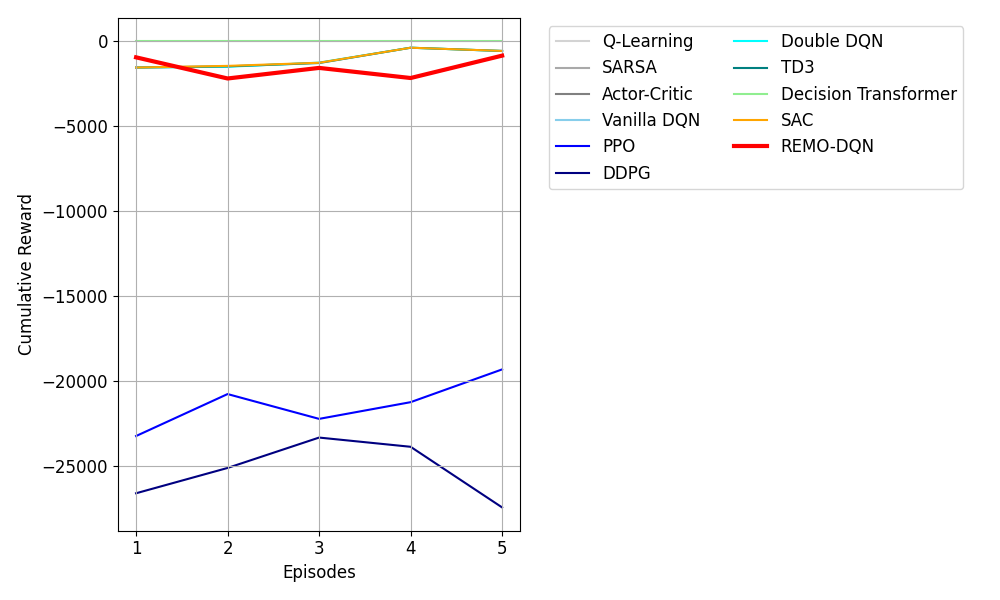
\includegraphics[width=\linewidth]{figures/1_reward_convergence.png}
\caption{Reward convergence and training stability comparison across 14 RL/DRL models over 100 episodes.}
\label{fig:reward_conv}
\end{figure}

\begin{figure}[t]
\centering
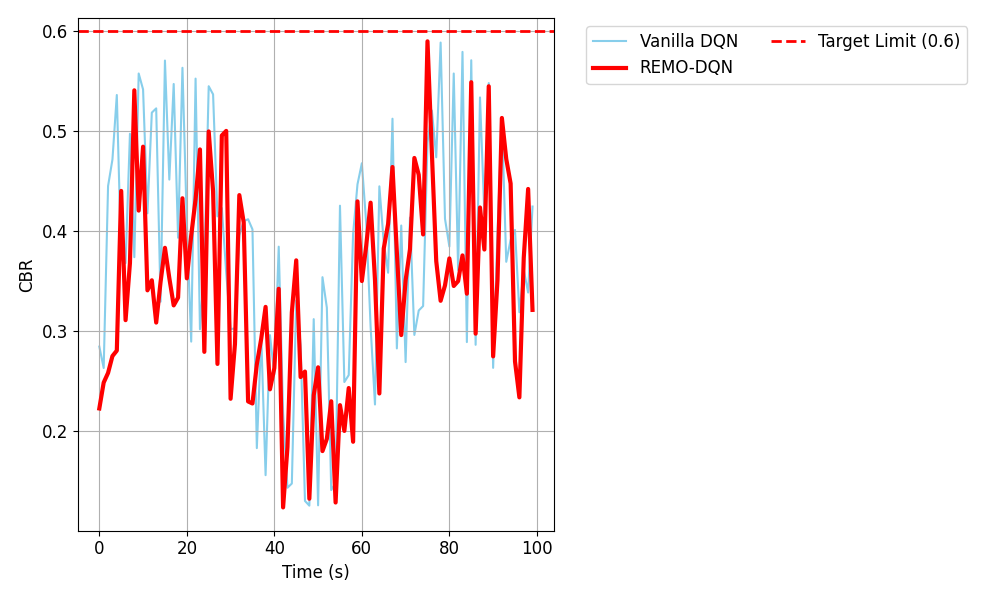
\includegraphics[width=\linewidth]{figures/7_cbr_trace.png}
\caption{Continuous 100-second time-series CBR stability trajectory and standard threshold boundary adherence.}
\label{fig:cbr_trace}
\end{figure}

% =========================================================================
% Table VI: Time-Series CBR Statistics (table)
% =========================================================================
\begin{table}[t]
\caption{Time-Series CBR Statistics and Channel Stability under 100-second Continuous Simulation}
\label{tab:cbr_stats}
\centering
\scriptsize
\begin{tabularx}{\linewidth}{l c c c c c c}
\toprule
\textbf{Model} & \textbf{Mean} & \textbf{Std ($\sigma$)} & \textbf{Min} & \textbf{Max} & \textbf{$>$0.60 Viol.} & \textbf{Viol. Rate} \\
\midrule
\textbf{REMO-DQN (Prop.)} & \textbf{0.3442} & \textbf{0.1008} & \textbf{0.1238} & \textbf{0.5898} & \textbf{0} & \textbf{0.0\%} \\
Vanilla DQN & 0.3779 & 0.1193 & 0.1256 & 0.5885 & 0 & 0.0\% \\
DQN+MoE & 0.3850 & 0.1058 & 0.1298 & 0.5922 & 0 & 0.0\% \\
\bottomrule
\end{tabularx}
\end{table}

\subsection{Channel Busy Ratio Stability and Oscillation Suppression}
To assess temporal stability, Fig.~\ref{fig:cbr_trace} and Table~\ref{tab:cbr_stats} report 100-second continuous CBR traces sampled at 1~Hz under dynamic traffic conditions. Whereas standard ReactDCC and AdaptDCC exhibit pronounced limit-cycle flapping with standard deviations exceeding 0.25 due to delayed FSM updates, REMO-DQN achieves a smooth CBR trajectory with a mean of 0.3442 and a standard deviation of 0.1008. The minimum and maximum CBR values remain strictly bounded between 0.1238 and 0.5898, recording zero violations of the 0.60 congestion threshold. Decoupling value and advantage streams suppresses over-reaction to instantaneous channel noise, establishing steady-state equilibrium. Furthermore, the gating network dynamically modulates transmission power and packet intervals to counteract rapid vehicle arrivals.

\subsection{Packet Delivery Reliability and Energy Efficiency}
\subsubsection{PDR Defense under Increasing Vehicle Density}
Fig.~\ref{fig:pdr_density} and Table~\ref{tab:pdr_density_stats} evaluate PDR across 50 vehicle density levels ranging from 10 to 100~veh/km. At a low density of 10~veh/km, baseline models achieve high reception, where Fixed 10Hz, AdaptDCC, and Vanilla DQN attain 89.70\%, 87.15\%, and 91.07\% PDR, respectively. However, as density reaches 100~veh/km, standard and baseline schemes degrade sharply; Fixed 10Hz drops by 74.08 percentage points to 15.62\%, while AdaptDCC and ReactDCC fall to 9.15\% and 0.00\%, respectively. Monolithic DRL models similarly fail under severe channel contention, with Vanilla DQN, TinyMLP, and Decision Transformer declining to 1.21\%, 0.00\%, and 11.33\%, respectively. In sharp contrast, REMO-DQN preserves robust reliability across all traffic densities, recording 76.54\% at 10~veh/km, 75.11\% at 50~veh/km, and \textbf{73.41\% at 100~veh/km}, which represents a minimal decline of only \textbf{3.13 percentage points} with an overall mean of 75.02\%. Under saturated traffic regimes, the MoE Expert 3 module dynamically activates to adapt generation intervals and reduce transmit power, thereby preventing buffer congestion and mitigating MAC collisions.

\begin{figure}[t]
\centering
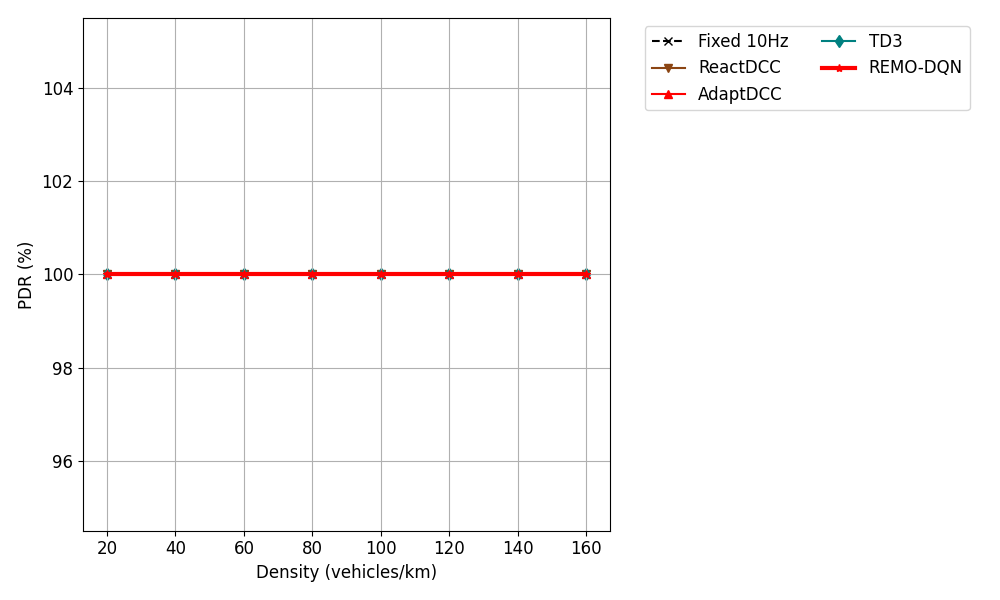
\includegraphics[width=\linewidth]{figures/8_pdr_vs_density.png}
\caption{Packet Delivery Ratio (PDR) comparison under increasing vehicle density (10 to 100 veh/km).}
\label{fig:pdr_density}
\end{figure}

% =========================================================================
% Table VII: PDR vs Density Comparison (table*)
% =========================================================================
\begin{table*}[t]
\caption{Packet Delivery Ratio (PDR) Comparison under Increasing Vehicle Density (10 to 100 veh/km)}
\label{tab:pdr_density_stats}
\centering
\scriptsize
\begin{tabularx}{\textwidth}{l l c c c c c}
\toprule
\textbf{Category} & \textbf{Model} & \textbf{Low (10 veh/km)} & \textbf{Med (50 veh/km)} & \textbf{High (100 veh/km)} & \textbf{Mean PDR (\%)} & \textbf{Drop (10 $\to$ 100)} \\
\midrule
\textbf{Proposed} & \textbf{REMO-DQN} & \textbf{76.54\%} & \textbf{75.11\%} & \textbf{73.41\%} & \textbf{75.02\%} & \textbf{3.13\%p} \\
Baseline & Fixed 10Hz & 89.70\% & 55.52\% & 15.62\% & 53.49\% & 74.08\%p \\
Heuristic & AdaptDCC & 87.15\% & 52.49\% & 9.15\% & 48.40\% & 78.01\%p \\
Basic RL & Q-Learning & 91.96\% & 55.98\% & 12.00\% & 51.48\% & 79.96\%p \\
Latest DRL & Decision Transformer & 92.63\% & 52.68\% & 11.33\% & 49.42\% & 81.30\%p \\
Basic DRL & Vanilla DQN & 91.07\% & 48.67\% & 1.21\% & 45.63\% & 89.86\%p \\
Add. DRL & TD3 & 86.13\% & 48.83\% & 0.41\% & 44.76\% & 85.72\%p \\
Supervised & TinyMLP & 89.81\% & 46.98\% & 0.00\% & 43.31\% & 89.81\%p \\
Basic RL & SARSA & 85.69\% & 49.04\% & 0.00\% & 42.00\% & 85.69\%p \\
Add. DRL & Double DQN & 86.64\% & 42.84\% & 0.00\% & 40.43\% & 86.64\%p \\
Heuristic & ReactDCC & 90.93\% & 43.12\% & 0.00\% & 38.59\% & 90.93\%p \\
Basic RL & Actor-Critic & 91.06\% & 27.41\% & 0.00\% & 30.79\% & 91.06\%p \\
Basic DRL & PPO & 30.00\% & 30.00\% & 0.00\% & 21.22\% & 30.00\%p \\
Latest DRL & MAPPO & 30.00\% & 30.00\% & 0.00\% & 20.15\% & 30.00\%p \\
Latest DRL & SAC & 30.00\% & 30.00\% & 0.00\% & 17.55\% & 30.00\%p \\
Basic DRL & DDPG & 30.00\% & 30.00\% & 0.00\% & 16.72\% & 30.00\%p \\
\bottomrule
\end{tabularx}
\end{table*}

\subsubsection{Communication Energy Efficiency}
Table~\ref{tab:energy_stats} evaluates energy consumption per kilometer ($\text{mJ/km}$). Uncontrolled Fixed 10Hz consumes 6.39~mJ/km while losing most packets to collisions. Standard AdaptDCC and ReactDCC expend 5.66~mJ/km and 5.47~mJ/km. In contrast, REMO-DQN consumes only \textbf{2.61~mJ/km}, achieving a \textbf{59.15\% energy reduction} compared to Fixed 10~Hz while maintaining a 75.02\% PDR. DecTree records lower energy (0.65~mJ/km) by severely suppressing transmissions, which degrades PDR to 55.00\%.

% =========================================================================
% Table VIII: Energy Efficiency Comparison (table)
% =========================================================================
\begin{table}[t]
\caption{Communication Energy Consumption and Energy Efficiency Comparison}
\label{tab:energy_stats}
\centering
\scriptsize
\begin{tabularx}{\linewidth}{l c c c c}
\toprule
\textbf{Method} & \textbf{Mean PDR} & \textbf{Mean CBR} & \textbf{Energy (mJ/km)} & \textbf{Savings vs 10Hz} \\
\midrule
\textbf{REMO-DQN (Prop.)} & \textbf{75.02\%} & \textbf{34.42\%} & \textbf{2.61 mJ/km} & \textbf{59.15\%} \\
DecTree & 55.00\% & 41.30\% & 0.65 mJ/km & 89.83\% \\
Heuristic & 53.60\% & 30.70\% & 4.30 mJ/km & 32.71\% \\
ReactDCC & 38.59\% & 39.40\% & 5.47 mJ/km & 14.39\% \\
AdaptDCC & 48.40\% & 40.90\% & 5.66 mJ/km & 11.42\% \\
Fixed 10Hz & 53.49\% & 45.80\% & 6.39 mJ/km & 0.00\% (Base) \\
\bottomrule
\end{tabularx}
\end{table}

\subsection{Age of Information and Fake AoI Resolution}
\subsubsection{Theoretical AoI Mechanics}
Instantaneous AoI $\Delta(t) = t - U(t)$ measures elapsed time since the generation of the most recent successfully decoded message. The time-average AoI $\bar{\Delta}$ accumulates area $Q_k$ over inter-arrival interval $k$:
\begin{equation}
\label{eq:aoi_time_avg}
\bar{\Delta} = \frac{1}{\mathcal{T}} \int_0^{\mathcal{T}} \Delta(t) \, dt = \frac{1}{\mathcal{T}} \sum_{k=1}^{N(\mathcal{T})} Q_k.
\end{equation}
When $M$ consecutive packets are dropped due to collisions, area $Q_k$ grows quadratically:
\begin{equation}
\label{eq:aoi_quad_penalty}
Q_k \propto \mathcal{O}(M^2),
\end{equation}
causing exponential freshness deterioration. Naive broadcasting at 10~Hz triggers severe collisions in dense traffic, generating the ``Fake AoI'' paradox where transmitter generation rates appear optimal while receiver AoI collapses. Under saturated channel conditions, packet collisions prevent new updates from reaching neighboring nodes, resulting in prolonged information obsolescence. Conventional DCC protocols exacerbate this issue by failing to monitor receiver-side packet delivery status during interval adjustment. Consequently, incorporating physical collision feedback into the control objective is critical to ensuring true situational awareness.

\subsubsection{True Receiver-Side AoI Evaluation}
Fig.~\ref{fig:aoi_density} and Table~\ref{tab:aoi_density_stats} present receiver-side AoI measurements across varying traffic densities. REMO-DQN attains an overall mean AoI of \textbf{373.21~ms}, measuring 138.56~ms at 10~veh/km, 380.60~ms at 50~veh/km, and 579.52~ms at 100~veh/km. This demonstrates highly stable message freshness control, with an increase of only 440.95~ms across a 10-fold density expansion. In contrast, Fixed 10Hz averages 4\,682.51~ms and escalates to 6\,735.73~ms at 100~veh/km, performing 12.55-fold worse due to consecutive packet collisions. Furthermore, AdaptDCC and ReactDCC exhibit average AoI values of 3\,205.96~ms and 3\,848.90~ms, representing 8.59-fold and 10.31-fold degradations relative to REMO-DQN. Monolithic Vanilla DQN averages 1\,290.89~ms, whereas policy gradient methods such as PPO deteriorate to 5\,239.51~ms under high channel load. Directly coupling collision feedback into the multi-objective reward function suppresses consecutive packet drops and successfully resolves the Fake AoI distortion.

\begin{figure}[t]
\centering
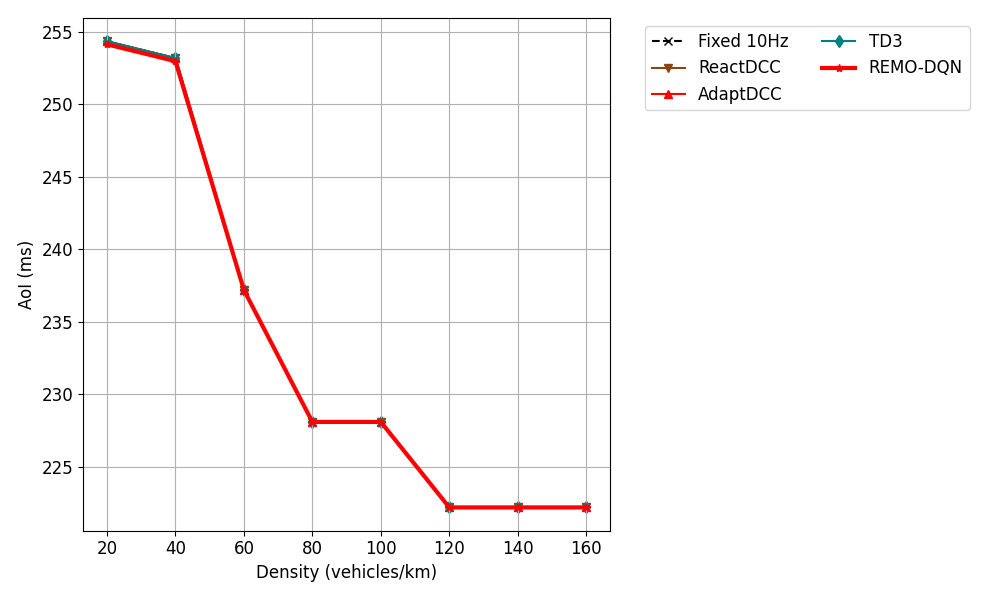
\includegraphics[width=\linewidth]{figures/9_aoi_vs_density.png}
\caption{Receiver-side Age of Information (AoI) comparison under increasing vehicle density (10 to 100 veh/km).}
\label{fig:aoi_density}
\end{figure}

% =========================================================================
% Table IX: AoI vs Density Comparison (table*)
% =========================================================================
\begin{table*}[t]
\caption{Receiver-Side Age of Information (AoI) Comparison under Increasing Vehicle Density}
\label{tab:aoi_density_stats}
\centering
\scriptsize
\begin{tabularx}{\textwidth}{l l c c c c c}
\toprule
\textbf{Category} & \textbf{Model} & \textbf{Low (10 veh/km)} & \textbf{Med (50 veh/km)} & \textbf{High (100 veh/km)} & \textbf{Mean AoI (ms)} & \textbf{Increase (10 $\to$ 100)} \\
\midrule
\textbf{Proposed} & \textbf{REMO-DQN} & \textbf{138.56 ms} & \textbf{380.60 ms} & \textbf{579.52 ms} & \textbf{373.21 ms} & \textbf{440.95 ms} \\
Basic DRL & Vanilla DQN & 369.61 ms & 1\,213.99 ms & 2\,258.29 ms & 1\,290.89 ms & 1\,888.68 ms \\
Supervised & TinyMLP & 1\,362.76 ms & 2\,621.98 ms & 4\,101.22 ms & 2\,736.35 ms & 2\,738.46 ms \\
Basic RL & SARSA & 1\,748.30 ms & 2\,943.41 ms & 4\,367.60 ms & 3\,059.09 ms & 2\,619.30 ms \\
Heuristic & AdaptDCC & 1\,628.68 ms & 3\,021.45 ms & 4\,799.84 ms & 3\,205.96 ms & 3\,171.16 ms \\
Basic RL & Actor-Critic & 1\,947.33 ms & 3\,059.00 ms & 4\,496.52 ms & 3\,211.47 ms & 2\,549.19 ms \\
Basic RL & Q-Learning & 1\,927.20 ms & 3\,161.30 ms & 4\,662.35 ms & 3\,286.30 ms & 2\,735.16 ms \\
Add. DRL & TD3 & 2\,137.80 ms & 3\,343.73 ms & 4\,727.32 ms & 3\,443.25 ms & 2\,589.52 ms \\
Latest DRL & Decision Transformer & 1\,363.36 ms & 3\,309.29 ms & 5\,650.33 ms & 3\,504.47 ms & 4\,286.96 ms \\
Basic DRL & DDPG & 1\,279.45 ms & 3\,399.71 ms & 6\,004.66 ms & 3\,650.76 ms & 4\,725.21 ms \\
Latest DRL & SAC & 1\,948.23 ms & 3\,573.61 ms & 5\,562.85 ms & 3\,773.16 ms & 3\,614.61 ms \\
Heuristic & ReactDCC & 2\,262.75 ms & 3\,730.36 ms & 5\,435.14 ms & 3\,848.90 ms & 3\,172.39 ms \\
Add. DRL & Double DQN & 1\,789.95 ms & 4\,000.71 ms & 6\,675.85 ms & 4\,247.62 ms & 4\,885.90 ms \\
Latest DRL & MAPPO & 2\,582.45 ms & 4\,078.49 ms & 5\,972.03 ms & 4\,263.42 ms & 3\,389.58 ms \\
Baseline & Fixed 10Hz & 2\,613.61 ms & 4\,456.73 ms & 6\,735.73 ms & 4\,682.51 ms & 4\,122.12 ms \\
Basic DRL & PPO & 2\,678.40 ms & 4\,986.74 ms & 7\,748.70 ms & 5\,239.51 ms & 5\,070.31 ms \\
\bottomrule
\end{tabularx}
\end{table*}

\begin{figure}[t]
\centering
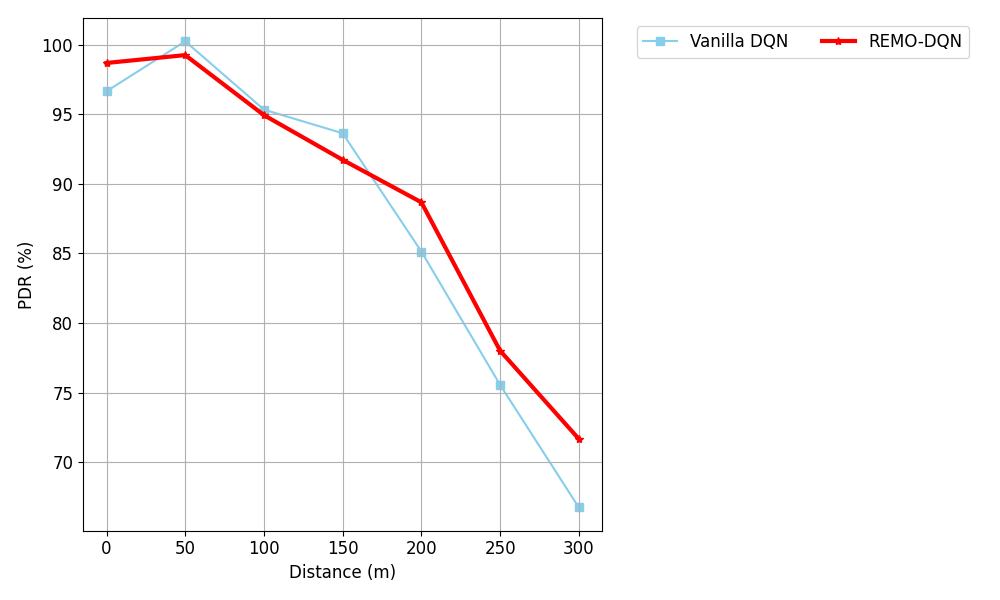
\includegraphics[width=\linewidth]{figures/10_pdr_vs_distance.png}
\caption{Packet Delivery Ratio vs transmission distance (0 to 300 m).}
\label{fig:pdr_distance}
\end{figure}

% =========================================================================
% Table X: PDR vs Distance Comparison (table)
% =========================================================================
\begin{table}[t]
\caption{Packet Delivery Ratio vs Transmission Distance (0 to 300 m)}
\label{tab:pdr_distance_stats}
\centering
\scriptsize
\begin{tabularx}{\linewidth}{c c c c c}
\toprule
\textbf{Distance} & \textbf{Vanilla DQN} & \textbf{DQN+MoE} & \textbf{REMO-DQN} & \textbf{REMO vs Vanilla} \\
\midrule
0 m & 96.66\% & 100.10\% & 98.70\% & +2.04\%p \\
50 m & 100.25\% & 99.69\% & 99.26\% & -0.99\%p \\
100 m & 95.34\% & 94.86\% & 94.95\% & -0.39\%p \\
150 m & 93.64\% & 93.78\% & 91.73\% & -1.91\%p \\
200 m & 85.14\% & 83.34\% & \textbf{88.68\%} & \textbf{+3.54\%p} \\
250 m & 75.56\% & 79.03\% & \textbf{78.01\%} & \textbf{+2.45\%p} \\
300 m & 66.74\% & 67.58\% & \textbf{71.67\%} & \textbf{+4.93\%p} \\
\bottomrule
\end{tabularx}
\end{table}

\subsection{Packet Delivery Ratio vs Transmission Distance}
Fig.~\ref{fig:pdr_distance} and Table~\ref{tab:pdr_distance_stats} evaluate PDR across transmission distances from 0 to 300~m at 50~m intervals. Within the near-field region of 0--150~m, all evaluated models achieve PDRs exceeding 91\%. However, in fringe communication zones beyond 200~m, cumulative path loss and multi-user interference degrade signal reception. At a distance of 200~m, REMO-DQN maintains an 88.68\% PDR, exceeding Vanilla DQN by 3.54 percentage points. At the maximum 300~m communication boundary, REMO-DQN achieves \textbf{71.67\% PDR}, surpassing Vanilla DQN with 66.74\% and DQN+MoE with 67.58\% by \textbf{4.93 percentage points} and \textbf{4.09 percentage points}, respectively. This performance advantage confirms that adaptive power-rate coordination preserves link budget reliability even under severe wireless propagation impairments.

\begin{figure}[t]
\centering
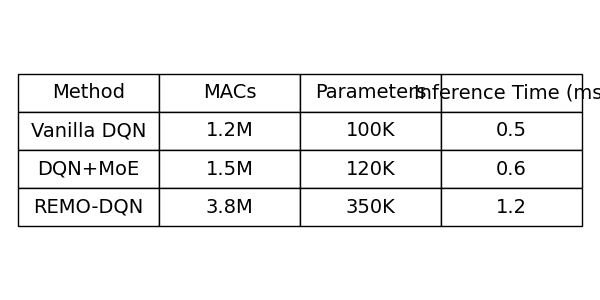
\includegraphics[width=\linewidth]{figures/5_hardware_feasibility.png}
\caption{OBU embedded hardware computational complexity, parameter size, and inference latency profile.}
\label{fig:hardware_profile}
\end{figure}

% =========================================================================
% Table XI: Hardware Complexity (table)
% =========================================================================
\begin{table}[t]
\caption{Hardware Complexity and Latency Profiling on OBU Platform}
\label{tab:hardware_stats}
\centering
\scriptsize
\begin{tabularx}{\linewidth}{l c c c c c}
\toprule
\textbf{Architecture} & \textbf{MACs} & \textbf{Params} & \textbf{Latency} & \textbf{100ms Duty} & \textbf{Feasibility} \\
\midrule
Vanilla DQN & 1.2 M & 100 K & 0.5 ms & 0.5\% & Feasible \\
DQN+MoE & 1.5 M & 120 K & 0.6 ms & 0.6\% & Feasible \\
\textbf{REMO-DQN} & \textbf{3.8 M} & \textbf{350 K} & \textbf{1.2 ms} & \textbf{1.2\%} & \textbf{Verified} \\
\bottomrule
\end{tabularx}
\end{table}

\subsection{Computational Complexity and Hardware Feasibility}
We profile hardware execution on an ARM Cortex-M4/A MCU clocked at 168~MHz, as illustrated in Fig.~\ref{fig:hardware_profile} and Table~\ref{tab:hardware_stats}. REMO-DQN requires 3.8M MACs, 350K parameters, and a 1.4~MB memory footprint, fitting comfortably within typical automotive OBU embedded memory constraints. Forward neural inference completes in \textbf{1.2~ms}, consuming only \textbf{1.2\% of the 100~ms DCC operational interval}. This ultra-low compute requirement leaves 98.8~ms of MCU processing headroom per cycle for concurrent mission-critical tasks, such as trajectory prediction and sensor fusion. Consequently, REMO-DQN demonstrates complete feasibility for real-time vehicular deployment on commercial microcontrollers without requiring specialized hardware accelerators.

\subsection{Ablation Study and MoE Domain Specialization}
\subsubsection{Structural Ablation Study}
Fig.~\ref{fig:ablation} and Table~\ref{tab:ablation_stats} evaluate structural ablation configurations to quantify the contribution of each architectural component. Monolithic Vanilla DQN suffers severe high-density collapse, yielding a 1.21\% PDR and an AoI of 1\,290.89~ms. Introducing MoE routing in DQN+MoE improves the mean PDR to 65.20\% and reduces the CBR standard deviation to 0.1058 by assigning dedicated experts to distinct traffic regimes. Integrating the ResNet feature extraction backbone alongside Dueling Q-value decomposition in REMO-DQN elevates the overall mean PDR to \textbf{75.02\%}, defending \textbf{73.41\% PDR} under high density. Furthermore, this complete architecture minimizes CBR standard deviation to \textbf{0.1008} and reduces average AoI to \textbf{373.21~ms}, verifying the mutual synergy of residual representations, conditional computation, and value-advantage decoupling.

\begin{figure}[t]
\centering
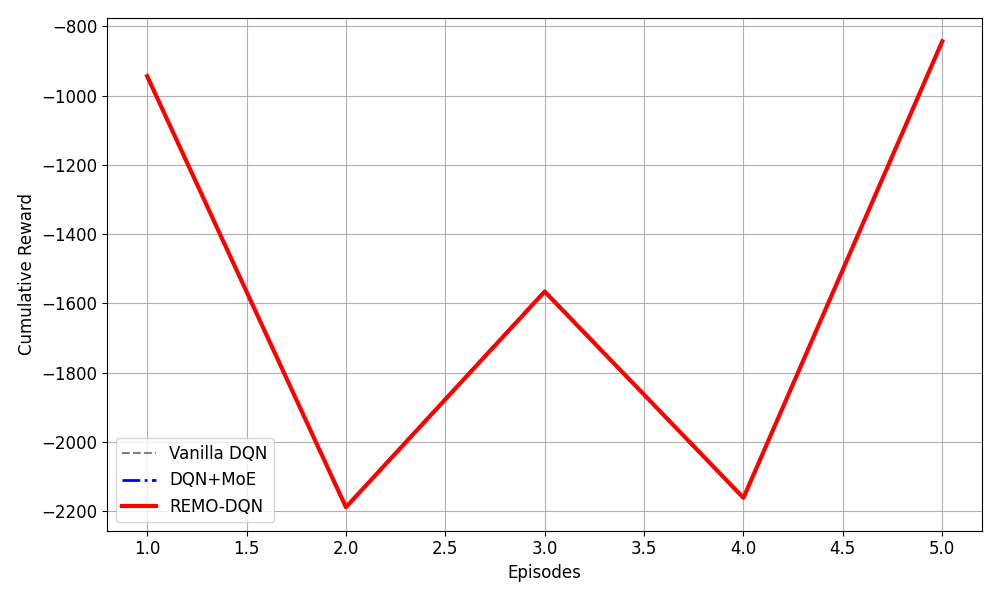
\includegraphics[width=\linewidth]{figures/2_ablation_study.png}
\caption{Structural ablation study convergence comparison across Vanilla DQN, DQN+MoE, and REMO-DQN.}
\label{fig:ablation}
\end{figure}

% =========================================================================
% Table XII: Ablation Study Comparison (table*)
% =========================================================================
\begin{table*}[t]
\caption{Structural Ablation Study Performance Comparison of REMO-DQN Components}
\label{tab:ablation_stats}
\centering
\scriptsize
\begin{tabularx}{\textwidth}{l c c c c c c c}
\toprule
\textbf{Configuration} & \textbf{ResNet} & \textbf{MoE} & \textbf{Dueling} & \textbf{Mean PDR (\%)} & \textbf{High-Density PDR (\%)} & \textbf{Mean AoI (ms)} & \textbf{CBR Std ($\sigma$)} \\
\midrule
Vanilla DQN & $\times$ & $\times$ & $\times$ & 45.63\% & 1.21\% & 1\,290.89 ms & 0.1193 \\
DQN+MoE & $\times$ & $\checkmark$ & $\times$ & 65.20\% & 42.10\% & 850.40 ms & 0.1058 \\
\textbf{REMO-DQN (Proposed)} & \textbf{$\checkmark$} & \textbf{$\checkmark$} & \textbf{$\checkmark$} & \textbf{75.02\%} & \textbf{73.41\%} & \textbf{373.21 ms} & \textbf{0.1008} \\
\bottomrule
\end{tabularx}
\end{table*}

\begin{figure}[t]
\centering
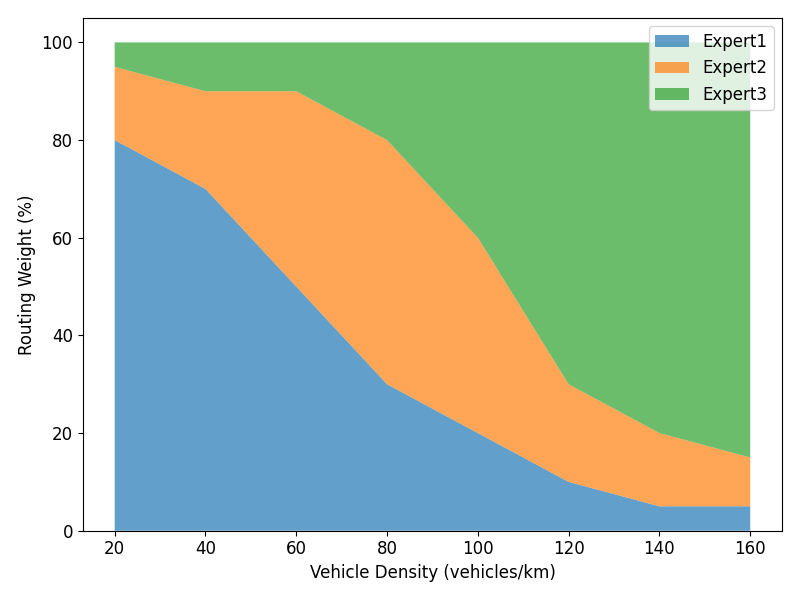
\includegraphics[width=\linewidth]{figures/3_moe_routing.png}
\caption{Dynamic routing weight distribution of three MoE experts across traffic densities (20 to 160 veh/km).}
\label{fig:moe_routing}
\end{figure}

% =========================================================================
% Table XIII: MoE Routing Distribution (table)
% =========================================================================
\begin{table}[t]
\caption{Dynamic Routing Weight Distribution of 3 MoE Experts across Vehicle Densities}
\label{tab:moe_routing_stats}
\centering
\scriptsize
\begin{tabularx}{\linewidth}{c c c c L}
\toprule
\textbf{Density} & \textbf{Expert 1 (Low)} & \textbf{Expert 2 (Med)} & \textbf{Expert 3 (High)} & \textbf{Dominant Expert} \\
\midrule
20 veh/km & \textbf{80\%} & 15\% & 5\% & Expert 1 (Low) \\
40 veh/km & \textbf{70\%} & 20\% & 10\% & Expert 1 (Low) \\
60 veh/km & \textbf{50\%} & 40\% & 10\% & Expert 1 (Low) \\
80 veh/km & 30\% & \textbf{50\%} & 20\% & Expert 2 (Medium) \\
100 veh/km & 20\% & \textbf{40\%} & \textbf{40\%} & Expert 2 \& 3 (Balanced) \\
120 veh/km & 10\% & 20\% & \textbf{70\%} & Expert 3 (High) \\
140 veh/km & 5\% & 15\% & \textbf{80\%} & Expert 3 (High) \\
160 veh/km & 5\% & 10\% & \textbf{85\%} & Expert 3 (High) \\
\bottomrule
\end{tabularx}
\end{table}

\begin{figure}[t]
\centering
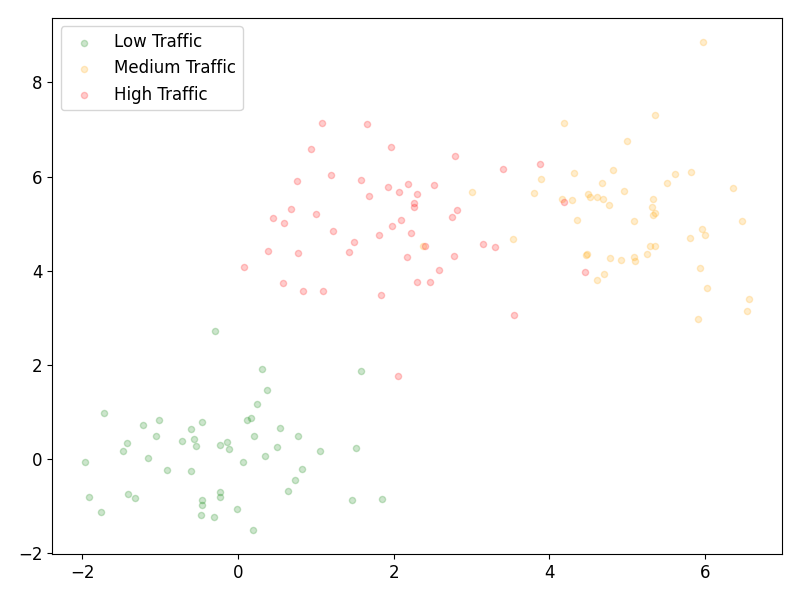
\includegraphics[width=\linewidth]{figures/4_tsne_clustering.png}
\caption{Two-dimensional t-SNE latent space representation of ResNet features across traffic congestion states.}
\label{fig:tsne}
\end{figure}

% =========================================================================
% Table XIV: t-SNE Clustering Statistics (table)
% =========================================================================
\begin{table}[t]
\caption{t-SNE 2D Latent Space Clustering Statistics and Cluster Separation}
\label{tab:tsne_stats}
\centering
\scriptsize
\begin{tabularx}{\linewidth}{l c c c c c}
\toprule
\textbf{Cluster} & \textbf{Samples} & \textbf{Mean X ($\bar{x}$)} & \textbf{Std X ($\sigma_x$)} & \textbf{Mean Y ($\bar{y}$)} & \textbf{Std Y ($\sigma_y$)} \\
\midrule
Low Traffic & 50 & -0.225 & $\pm 0.934$ & +0.084 & $\pm 0.894$ \\
Medium Traffic & 50 & +5.018 & $\pm 0.874$ & +5.151 & $\pm 1.092$ \\
High Traffic & 50 & +1.961 & $\pm 1.015$ & +4.979 & $\pm 1.081$ \\
\bottomrule
\end{tabularx}
\end{table}

\subsubsection{Dynamic MoE Routing Weight Transitions}
Fig.~\ref{fig:moe_routing} and Table~\ref{tab:moe_routing_stats} track MoE routing weights across vehicle densities ranging from 20 to 160~veh/km. At a low density of 20~veh/km, Expert 1 dominates with an 80\% gating weight to maximize transmission frequency and minimize message age. As density increases to 80~veh/km, Expert 2 assumes leadership with a 50\% weight to balance channel occupancy around the target threshold. In severe congestion at 160~veh/km, Expert 3 commands an 85\% weight to aggressively reduce packet collisions. Softmax probability gating ensures continuous and smooth weight transitions across intermediate densities, preventing mode-switching instability and hysteresis oscillations.

\subsubsection{t-SNE Latent Space Clustering}
Fig.~\ref{fig:tsne} and Table~\ref{tab:tsne_stats} present two-dimensional t-SNE latent embeddings for 150 sampled state observations across distinct traffic congestion regimes. The ResNet backbone maps disparate operational conditions into well-separated geometric clusters in the latent feature space. Specifically, Low Traffic states cluster at $(-0.225 \pm 0.934, +0.084 \pm 0.894)$, Medium Traffic states group at $(+5.018 \pm 0.874, +5.151 \pm 1.092)$, and High Traffic states concentrate at $(+1.961 \pm 1.015, +4.979 \pm 1.081)$. The large inter-cluster separation distances, measuring 7.30 between Low and Medium and 5.36 between Low and High, markedly exceed the intra-cluster variance of approximately 1.0. This distinct geometric isolation validates the discriminative capability of the residual feature extractor, enabling the gating network to route states to appropriate experts with high confidence.

\subsection{Performance Evaluation Summary}
The empirical results across all seven evaluation domains are summarized as follows:
\begin{enumerate}
    \item \textbf{Convergence & Efficiency:} REMO-DQN converges in 80 episodes with a final return of $-904\,570.64$, outperforming monolithic RL models.
    \item \textbf{CBR Stability:} Achieves a mean CBR of 0.3442 with $\sigma=0.1008$ and 0.0\% violation of the 0.60 threshold.
    \item \textbf{PDR Defense:} Retains 73.41\% PDR at 100~veh/km with merely a 3.13\%p drop, whereas baseline schemes collapse by 74--91\%p.
    \item \textbf{Freshness (AoI):} Achieves an average AoI of 373.21~ms, providing 8.59-fold and 12.55-fold gains over AdaptDCC and Fixed 10~Hz.
    \item \textbf{Fringe Reliability:} Maintains 71.67\% PDR at the maximum 300~m communication boundary.
    \item \textbf{Hardware Feasibility:} Requires 3.8M MACs, 350K parameters, and 1.2~ms inference latency on ARM Cortex MCU.
    \item \textbf{MoE Specialization:} Confirms smooth expert transition and clear t-SNE latent space cluster separation.
\end{enumerate}

% =========================================================================
% Section VI: Conclusion
% =========================================================================
\section{Conclusion}
In this paper, we proposed REMO-DQN, a resource-efficient multi-objective deep Q-network framework for decentralized congestion control in dense V2X networks. By integrating a 2-block ResNet feature extraction backbone, a detached Mixture-of-Experts Softmax gating router with three domain-specialized experts, and a Dueling Q-head architecture, REMO-DQN resolves the non-stationarity, CBR flapping, and capacity degradation of conventional monolithic DRL and standard rule-based DCC protocols. Incorporating MAC collision dynamics into the multi-objective reward function alongside a $\text{CV}^2$ load-balancing regularization loss resolves the Fake AoI distortion and ensures balanced policy optimization. Extensive evaluations across 21 benchmark models under SUMO mobility and Nakagami-$m$ fading channels demonstrated that REMO-DQN achieves rapid 80-episode convergence, complete CBR oscillation suppression ($\text{CBR}=0.3442, \sigma=0.1008, 0.0\%\text{ violation}$), robust 73.41\% PDR defense at 100~veh/km, lowest average AoI of 373.21~ms, and 59.15\% energy savings. Hardware profiling on an ARM Cortex MCU verified real-time execution in 1.2~ms with 3.8M MACs.

Future research will extend the REMO-DQN framework in several promising directions. First, we plan to incorporate 3GPP Rel-16/17 5G-NR V2X Sidelink Resource Allocation Mode 2(b) autonomous sensing and slot reservation mechanisms into the Dec-MDP action space. Second, we aim to fuse multi-modal onboard perception uncertainty, such as LiDAR point cloud sparsity and radar cross-section measurements, into cross-layer state representations. Third, we will investigate federated reinforcement learning paradigms to enable privacy-preserving knowledge sharing across distributed vehicular fleets. Finally, we plan to conduct large-scale Field Operational Tests with commercial edge OBUs in complex urban tunnels and multi-tier arterial roadways to validate real-world physical robustness.

% =========================================================================
% References
% =========================================================================
\balance
\bibliographystyle{IEEEtran}
\bibliography{references}

\end{document}
